\documentclass[11pt]{jarticle}
\usepackage{ITCannual}
\usepackage{amsmath}
\usepackage{amssymb}
\usepackage{times}
\usepackage[dvipdfmx]{graphicx}

%\usepackage[style=numeric]{biblatex}

\title{データ科学研究部門 研究報告}
\author{小林博樹, 鈴村豊太郎, 空閑洋平, Parajuli Laxmi Kumar, 河村光晶, 川瀬純也, 華井雅俊,\\
\textbf{Li Zihui, 上坂怜生, 石川正俊, 早川智彦, 黄守仁, 末石智大, 宮下令央, 田畑智志}}

\begin{document}
\maketitle

\section{データ科学研究部門 概要(昨年の文言)}
データ科学研究部門では、2022度、教授4名(特任教授1名)、准教授3名(特任准教授2名)、講師4名(特任講師4名)、助教5名(特任助教3名)、研究員1名(特任研究員1名)が在籍した。同部門のメンバーは専任教員と特任教員の2つのグループから成る。専任教員はそれぞれが独立して研究活動を行うグループで、特任教員は石川特任教授を中心とする石川グループ研究室である。

% \subsection{専任教員グループの研究テーマ}
%
% \begin{quote}
% \begin{itemize}
% \item 計算機を介した人と生態系のインタラクションの研究(小林)
% \item 大規模グラフニューラルネットワークと様々な実社会問題への応用(鈴村)
% \item データセンタハードウェアへのソフトウェア脆弱試験の適応(空閑)
% \item Title (Kumar)
% \item Title (河村)
% \item データ駆動型知能に基づくアーバンコンピューティング(姜)
% \item 野生動物ワイヤレスセンサネットワーク実証実験基盤構築に向けた研究(川瀬)
% \item グラフニューラルネットワークとその物性予測問題への応用に関する研究(華井)
% \item Title (Zihui)
% \end{itemize}
% \end{quote}

%\subsection{石川研究室全体の研究活動概要}
%\subsection{研究報告(石川グループ研究室)}

%  センサやロボットはもちろんのこと、社会・心理現象等も含めて、現実の物理世界は、原則的に並列かつリアルタイムの演算構造を有している。その構造と同等の構造を工学的に実現することは、現実世界の理解を促すばかりでなく、応用上の様々な利点をもたらし、従来のシステムをはるかに凌駕する性能を生み出すことができ、結果として、まったく新しい情報システムを構築することが可能となる。本研究室では、特にセンサ情報処理における並列処理と高速・リアルタイム性を高度に示現する研究として、以下4つの分野での研究を行っている。また、新規産業分野開拓にも力を注ぎ、研究成果の技術移転,共同研究,事業化等を様々な形で積極的に推進している。

% 五感の工学的再構成を目指したセンサフュージョンの研究では、理論並びにシステムアーキテクチャの構築とその高速知能ロボットの開発、その応用としての新規タスクの実現、特に、視・触覚センサによるセンサ情報に基づく人間機械協調システムの開発を行っている。

% ダイナミックビジョンシステムの研究では、高速ビジョンや動的光学系に基づき運動対象の情報を適応的に取得する基礎技術の開発、特に、高速光軸制御や可変形状光学系の技術開発やトラッキング撮像に関する応用システムの開発を行っている。

% 高速三次元形状計測や高速質感計測など、並列処理に基づく高速画像処理技術 (理論、アルゴリズム、デバイス) 開発とその応用システムの実現を目指すシステムビジョンデザインの研究では、特に高速画像処理システムの開発、高速性を利用した新しい価値を創造する応用システムの開発を行っている。

% 実世界における新たな知覚補助技術並びにそれに基づく新しい対話の形の創出を目指すアクティブパーセプション技術の構築とその応用に関する研究では、特に各種高速化技術を用いた能動計測や能動認識を利用した革新的情報環境・ヒューマンインタフェイスの開発を行っている。



\section{データ科学研究部門 教員研究活動}

\subsection{計算機を介した人と生態系のインタラクションの研究(小林 博樹)}

本研究室は計算機を介した人と生態系のインタラクションの研究の行っている。これまで人間を対象とした知能情報学の見地を、多様で複雑な実世界の生物・環境・地理学・獣医学領域へ応用・発展させる研究である。研究内容はコンピュータ科学、環境学、メディアアート、など多岐に亘っており、特に、計算機を介した人と生態系のインタラクションHCBI(Human-Computer-Biosphere Interaction)の概念を情報学分野で発表し、このテーマを中心に、環境問題の解決を目的として、国内外で研究活動を独自に行ってきた。古典的なコンピュータ科学では、HCI(Human-Computer Interaction)が主要な研究領域の1つとなるが、本研究室はこの研究領域を地球環境にまで拡大すべく、人間と生態系の調和あるインタラクションを実現するシステムを提案し「時空間スケールの大きい環境問題を自律的に解決する情報基盤技術」として、そのフィールドでの実証実験を試みている。つまり、コンピュータ科学の分野では人間が活動する地理空間を対象とした研究が中心であったが、本研究室は人間が活動していない、情報通信技術の応用が困難な地理空間を対象にした情報デザインと野生動物IoTの研究を行っている。このように本研究室は、情報工学をベースとして、特に計算機を用いて生態系と人間のインタラクションを専門として実績をあげている。2022年度から科学技術振興機構の創発的研究支援事業として業務を実施している。
 
%  \begin{雑誌論文}{1}
 \bibitem{kobayashi1-1}
 Wenjing Li, Xiaodan Shi, Dou Huang, Xudong Shen, Jinyu Chen, Hill Hiroki Kobayashi, Haoran Zhang, Xuan Song, Ryosuke Shibasaki,  "PredLife: Predicting Fine-Grained Future Activity Patterns ", IEEE Transactions on Big Data 9(6) 1658-1669.

 \bibitem{kobayashi1-2}
 Wenjing Li, Haoran Zhang, Jinyu Chen, Peiran Li, Yuhao Yao, Xiaodan Shi, Mariko Shibasaki, Hill Hiroki Kobayashi, Xuan Song 0001, Ryosuke Shibasaki,  "Metagraph-Based Life Pattern Clustering With Big Human Mobility Data", IEEE Trans. Big Data 9(1) 227-240.
 
 \end{雑誌論文}

 \begin{査読付}{1}
 \bibitem{kobayashi2-1}
 Usman Haider, Muhammad Hanif, Hill Hiroki Kobayashi, Laxmi Kumar Parajuli, Daisuké Shimotoku, Ahmar Rashid, Sonia Safeer, "Bioacoustics Signal Classification Using Hybrid Feature Space with Machine Learning", Proceedings of 15th International Conference on Computer and Automation Engineering(ICCAE), 2023.  

 \bibitem{kobayashi2-2}
 Leo Uesaka, Ambika Prasad Khatiwada, Daisuk\'e Shimotoku, Laxmi Kumar Parajuli, Manish Raj Pandey, Hill Hiroki Kobayashi, "Applications of Bioacoustics Human Interface System for Wildlife Conservation in Nepal", Proceedings of 2023 International Conference on Human-Computer Interaction (HCII 2023), 2023.  

 \end{査読付}



% %半ページから1ページが文量

\subsection{深層学習に基づく推薦システムに関する研究(鈴村 豊太郎)}

本節では2023年度の鈴村豊太郎の研究活動について報告する。鈴村は、グラフニューラルネットワーク(GNN)、大規模言語モデル(LLM)などの深層学習を基盤にした推薦システムの研究を進めている。

推薦システムは、ユーザの好みやアイテム行動パターンなどをモデル化し、どのようなアイテムを購入するかを予測する問題であり、現実世界のあらゆるサービスに推薦システムが用いられていると言っても過言ではない。本年度は、地理空間領域、ニュース領域、求人マッチング領域における推薦システム、およびLLMベースの推薦システムの研究を進めている。

 時空間における推薦システムでは、自動車の走行軌跡データに基づき次に訪問する地点(Point-of-Interest, POI)を予測するPOI推薦において、ユーザの空間的・時間的特徴をそれぞれグラフ構造として表現し、ユーザの行動パターンを捉えるトランスフォーマベースのモデルアーキテクチャ Mobility Graph Transformer (MobGT) を提案した。この研究成果は地理情報空間におけるトップカンファレンスである国際学会 ACM SIGSPATIAL'23 に採択され、発表を行った(\cite{mobgt})。これらはトヨタ自動車との共同研究の成果でもある。

 ニュース領域における推薦モデルでは、全ユーザの記事閲覧行動データからなる Global News Graph と記事の内容から生成された Global Entity Graph を生成し、個別のユーザの閲覧履歴と組み合わせることで、ユーザの潜在的な記事閲覧パターンを捉える記事推薦システムモデル GLORY を提案した。この論文は国際学会 ACM RecSys 2023 に採択され、Best Full Paper Runner-Up Award 及び Best Student Paper Award を受賞した(\cite{glory})。
また、新しい記事が常に追加されるニュースサイトにおいては、過去に掲載された記事がすぐに閲覧されなくなるため、これらの記事の鮮度がニュース記事の推薦において重要である。そこで、この記事の鮮度をその内容や人気度などかを考慮して予測し、ユーザにより適切な記事を推薦するモデルを提案する。ニュース領域では日本経済新聞社との共同研究を進めている。

 求人マッチング領域では、ユーザの嗜好のみに基づく他の一般的な推薦システムとは異なり、求人側の意向も加味して、全体的な市場のマッチングを最大化する必要がある。そこで、マッチング数を報酬とした強化学習モデルを用いることで、end-to-end でマッチング数を最大化する手法を提案した。さらに、ユーザと求人に対する実際のマッチング数の少なさを補うために、ユーザの求人への応募、マッチングを二部グラフとして表現し、GNNモデル、グラフ拡張によって精度を向上させる手法を提案した。この研究成果は、それぞれ人工知能学会全国大会 (\cite{job-jsai})
)及び AAAI Workshop (\cite{job-aaai}) に採択され発表を行い、現在ACMの情報抽出関連の国際会議 ACM SIGIR 2024 に投稿、査読中である。また、昨年度に引き続きエス・エム・エス社との共同研究を進めており、実サービスでの検証に向けシミュレーションによる評価だけでなく A/B テストも実施した。

 大規模言語モデル LLM (Large Language Model) ベースの推薦システムでは、数値情報のエンコーティングに関する研究を行っている。推薦モデルでは、価格や数量など数値自体が意味を持つことが多いが、現状のLLMでは数字情報を理解することが苦手であり、推薦システムへの応用のネックとなっている。そこで、既存の推薦システム用の基盤モデルに対し、pre-training 時に加算など補助的な算術演算のタスクを行うことで、数値に関する表現を部分的に捉えることを示した。この研究成果は、AAAI Workshop にて採択、発表された (\cite{num-aaai})。

 また、前述の地理空間推薦システムにおいて、POI の情報としてテキストに、画像などマルチモーダルな情報を活用した POI推薦フレームワークを設計し、プロトタイプを実装、性能評価を続けている。ユーザが訪問した地点のジャンル、紹介文、写真をそれぞれテキストとして表現し、LLMベースの時系列推薦モデルを用いてより高精度なPOI推薦を実現することも目指している。

また、SIGIR 2023 \cite{sigir}, WWW 2023 \cite{kg-kp}の論文に関しては2022年度年報に報告済みであり詳細を割愛するが、2023年度に発表を行ったのでこちらに触れておく。

学会活動としてはAAAI 2024の Organizing Chairs として Sponsor Chairを務めた。また、2023年度から人工知能学会における理事を務め、2024年5月開催の人工知能領域における国際シンポジウム isAI 2024 (The 16th JSAI International Symposia on AI)の委員長を務めて、学会の開催準備を進めている。



%%%% 以下、2022年度

% 本節では2022年度の鈴村豊太郎の研究活動について報告する。 鈴村は、 グラフ構造に対するニューラルネットワークを用いた表現学習 Graph Neural Network (以下、GNNと呼ぶ)の基礎研究及び応用研究に取り組んでいる。 グラフ構造は、 ノードと、 ノード同士を接続するエッジから構成されるデータ構造である。 インターネット上における社会ネットワーク、 購買行動、 サプライチェーン、 金融における決済データ、 交通ネットワーク、 蛋白質相互作用・神経活動・DNAシーケンス配列内の依存性、 物質の分子構造、 人間の骨格ネットワーク、 概念の関係性を表現した知識グラフなど、 グラフ構造として表現できる応用先は枚挙に暇がない。
% \par
% 当該研究領域における研究として、時系列・動的に変化する大規模グラフに対するGNNモデルの研究を行った。
% 動的グラフに対応するGNNモデルはすでに数多く提案されているが、いずれも短期的なデータの変化しか考慮されておらず、実世界で扱われている長期的なグラフデータでは長期的なコンテキストを捉えることができない問題が潜在的に存在していた。この問題に対して、時間幅が非常に長いグラフデータの性質も捉えることができる Spectral Waveletを提案した(AAAI 2023 \cite{aaai-deft}, Transactions on Machine Learning Research (TLMR) \cite{feta})。また、知識グラフ上で足りない関係性を補完する手法を評価する方法として トポロジカルデータ解析(Topological Data Analysis) における Persistent Homologyの概念を用いて効率的に評価する手法を提唱した(WWW 2023 \cite{kg-kp})。
% % 当該研究領域における研究として、時系列・動的に変化する大規模グラフに対するGNNモデルの研究を行った。実世界では時間幅が非常に長いデータを扱うこともあるが既存の動的グラフへのGNNの研究ではそのような点を考慮していない。この問題に対して、学習可能な Spectral Waveletを提案し、AAAI 2023 \cite{aaai-deft}, WWW 2023 \cite{deft}、 TLMR \cite{feta}に採択された。

% GNNに関する応用研究も進めている。金融領域においては不正検出に関するGNNモデルの検証を行い、取引ネットワークをヘテロジニアスなグラフ構造に拡張することによりモデル性能の向上を達成した(KDD'22 MLG Workshop \cite{eth-gnn})。マテリアルズ・インフォマティクスの分野においては、情報基盤センターの芝隼人先生とガラス物質の形成過程モデルに対して高精度なGNNモデルを提案し\cite{botan}、また当該分野における本質的な問題に対する手法として、インバランスなデータの問題を解消するための手法 \cite{xsig-limin}および外挿のためのモデル構築を行った\cite{xsig-takashige}。E-Commerceの領域においては知識グラフを用いた商品推薦手法を提案した (ACM SIGIR 2023 \cite{sigir})。

% また、理論モデルの実世界への検証と応用サイドから意味のある研究テーマを発掘するため、企業との共同研究とも進めている。まず、自動車の走行軌跡データから次の位置や経路を予測し、ロケーションリコメンデーションなどに応用するための手法をトヨタ自動車と探求している。走行軌跡データは緯度・経度及び時刻のシーケンスデータとなるが、それを用いると運転行動パターンを捉えることができる。
% % まずシーケンスデータからグラフ構造を構築し、そのグラフ構造からGraphormerというニューラルネットワークモデルを走行軌跡データのパターンを捉えられるようなニューラルネットワークのモデルを提案した。
% この行動パターンを捉えるために、シーケンスデータをグラフ構造として表現し、Graphormerをベースにした新たなモデルを提案し、他の既存手法よりも高い精度でパターンを予測することを確認した (ECML-PKDD \cite{stgtrans} 査読中)。
% % この新たなモデルを他の既存手法と比較し、より高い精度で走行パターンを予測する事を確認した。本研究の成果を ECML-PKDD \cite{stgtrans}に提出した。
% 来年度はモビリティにおける様々な領域に応用できるように、走行軌跡データや実世界の地図データなどから事前学習モデルを構築する予定である。また、その他に都市全体の二酸化炭素排出量を抑制するために交通流を分散するための手法をこれらの事前学習モデルと深層強化学習を用いて設計・実装する予定である。

% また、エス・エム・エス社との共同研究では、介護や医療領域における人材紹介の推薦システムに関する研究を行った。超高齢化社会に突入する中、介護や医療領域における人材不足は深刻であり、より精度の高い人材マッチングが不可欠である。この問題に対して、深層強化学習を用いた人材マッチング数の最適化手法を提案し、特定の求職者・事業者側に偏ってしまう従来の推薦・マッチング手法に対して、偏りを解消できることを確認した (人工知能学会\cite{sms} 6月発表予定)。来年度に関しては更に実データでの検証を進め、企業側での要望を取り入れ、実ビジネスが持つ制約条件を取り入れた最適化モデルを提案していく予定である。また、モデルにおいて求職者と求人側での動的な二部グラフの関係性及び知識グラフを用いてより精度高いモデルを構築していく予定である。

%  日本経済新聞社(以下、日経)との共同研究も2022年10月から開始している。日経ではニュースサイトにおける記事に対してより高度な機械学習による推薦システムを目指しており、2022年度は日経側での問題設定やデータの理解を図り、研究テーマの設定に主に取り組んだ。2023年度は推薦問題や広告配信など様々な領域に応用できるように、ユーザーの行動モデルを統一的に表現する事前学習モデルを構築するべく、自己教師付き学習 (Self-Supervised Learning)を用いた手法を設計・実装する予定である。

%  また、GNNの概要と最新研究動向に関する記事を人工知能学会誌\cite{jsai-gnn}に寄稿し、Federated Learning(連合学習)の英語書籍向けに Federated Learningを用いた金融不正検知に関する手法を執筆した\cite{fl-book}。mdxプロジェクトに関する第一弾の国際学会論文として IEEE CBDCom\cite{mdx}にて論文発表を行った。


% % How Expressive are Transformers in Spectral Domain for Graphs? \cite{feta}
% % Learnable Spectral Wavelets on Dynamic Graphs to Capture Global Interactions \cite{deft}
% % Can Persistent Homology provide an efficient alternative for Evaluation of Knowledge Graph Completion Methods? \cite{kg-kp}


% % Spatio-Temporal Meta-Graph Learning for Traffic Forecasting \cite{megacrn}

% % Ethereum Fraud Detection with Heterogeneous Graph Neural Networks \cite{eth-gnn}

% % Federated Learning for Collaborative Financial Crimes Detection \cite{fl-book}



% %  本節では2021 年度の鈴村豊太郎の研究活動について報告する。 2021年4月に本学に着任し、 グラフ構造に関するニューラルネットワークを用いた表現学習 Graph Neural Network (以下、GNNと呼ぶ)の基礎研究及びその様々な応用研究に取り組んでいる。 グラフ構造は、 ノードと、 ノード同士を接続するエッジから構成されるデータ構造である。 インターネット上における社会ネットワーク、 購買行動、 サプライチェーン、 金融における決済データ、 交通ネットワーク、 蛋白質相互作用・神経活動・DNAシーケンス配列内の依存性、 物質の分子構造、 人間の骨格ネットワーク、 概念の関係性を表現した知識グラフなど、 グラフ構造として表現できる応用先は枚挙に暇がない。
% % \par
% % 当該研究領域において、時系列・動的に変化する大規模グラフに対するGNNモデルの研究を行った。分散計算環境においてスケールするGNNモデルを提唱し、その成果は高性能計算分野におけるトップカンファレンスSC2021\cite{suzumura-sc2021}に採択された。 また、金融領域における不正検知手法として、TransformerアーキテクチャをベースにしたGNN手法を提案し、国際会議 IEEE SMDS 2021\cite{suzumura-smds21}に採択された。 また、 GNNに関する招待講演\cite{suzumura-canon2021}を行った。

% % これらの研究に続いて、推薦システムへのGNNモデルに関する研究を開始している。実データ・実問題に基づいた、社会実装を見据えた研究を進めるべく、医療・介護領域における人材推薦としてエス・エム・エス社、自動車における経路推薦としてトヨタ社と共同研究を2023年4月から本格的に開始する。また、国立研究開発法人物質・材料研究機構NIMSが主導する「マテリアル先端リサーチインフラ」プロジェクトの本学拠点の一貫で、材料情報科学 Materials Informaticsへの研究も開始している。
% %  データ科学・データ利活用のためのクラウド基盤 mdx プロジェクトにおいて、 今年度は 課金付き運用開始に向けたシステム拡張、スポットVM、データ共有機構(Platform-as-a-Service)に向けた設計を進めた。 また、 mdxに関する講演活動を国内外において行った\cite{suzumura-axies2021、suzumura-nanotec2021、 suzumura-nci2021}。 mdxの論文においては、国際会議IEEE IC2E2022(10th IEEE International Conference on Cloud Engineering) に2022年3月末に投稿した。 
% % %\cite{suzumura-mdx2022}においても論文を公開した。


% 




% % 
% % bibitem を作る
% \begin{雑誌論文}{1}
% \bibitem{feta}
% Bastos, Anson, Abhishek Nadgeri, Kuldeep Singh, Hiroki Kanezashi, Toyotaro Suzumura, and Isaiah Onando Mulang, "How Expressive Are Transformers in Spectral Domain for Graphs?", Transactions on Machine Learning Research (TMLR) ISSN 2835-8856, Journal of Machine Learning Research, 2022.
% \end{雑誌論文}


\begin{査読付}{5}

\bibitem{mobgt}
Xiaohang Xu, Toyotaro Suzumura, Jiawei Yong, Masatoshi Hanai, Chuang Yang, Hiroki Kanezashi, Renhe Jiang, and Shintaro Fukushima. 2023. Revisiting Mobility Modeling with Graph: A Graph Transformer Model for Next Point-of-Interest Recommendation. In Proceedings of the 31st ACM International Conference on Advances in Geographic Information Systems (SIGSPATIAL '23). Association for Computing Machinery, New York, NY, USA, Article 94, 1–10.

\bibitem{glory}
Boming Yang, Dairui Liu, Toyotaro Suzumura, Ruihai Dong, and Irene Li. 2023. Going Beyond Local: Global Graph-Enhanced Personalized News Recommendations. In Proceedings of the 17th ACM Conference on Recommender Systems (RecSys '23). Association for Computing Machinery, New York, NY, USA, 24–34.

\bibitem{sigir}
Md Mostafizur Rahman, Daisuke Kikuta, Satyen Abrol, Yu Hirate, Toyotaro Suzumura, Pablo Loyola, Takuma Ebisu and Manoj Kondapaka, "Exploring 360-Degree View of Customers for Lookalike Modeling",  SIGIR'23 (The 46th International ACM
SIGIR Conference on Research and Development in Information
Retrieval) 

\bibitem{kg-kp}
Anson Bastos, Kuldeep Singh, Abhishek Nadgeri, Johannes Hoffart, Toyotaro Suzumura, Manish Singh,
"Can Persistent Homology provide an efficient alternative for Evaluation of Knowledge Graph Completion Methods?"
In proceedings of The Web Conference (WWW), 2023.

\bibitem{job-aaai}
Waki, Satoshi, Toyotaro Suzumura, and Hiroki Kanezashi. "Optimizing Matching Markets with Graph Neural Networks and Reinforcement Learning." In Workshop on Recommendation Ecosystems: Modeling, Optimization and Incentive Design, AAAI 2024.

\bibitem{num-aaai}
Putra, Refaldi, and Toyotaro Suzumura. "On the Role of Numerical Encoding in Foundation Model of Sequential Recommendation with Sequential Indexing." In Workshop on Recommendation Ecosystems: Modeling, Optimization and Incentive Design. 2024, AAAI 2024


\bibitem{job-jsai}
脇聡志, 鈴村豊太郎, 金刺宏樹, 華井雅俊, 小林秀. "強化学習によるマッチング数を最大化するジョブ推薦システム." 人工知能学会全国大会論文集 第 37 回 (2023), 一般社団法人 人工知能学会, 2023.
\end{査読付}

% \begin{著書}{2}

% \bibitem{fl-book}
% Toyotaro Suzumura, Yi Zhou, Ryo Kawahara, Nathalie Baracaldo, Heiko Ludwig,
% "Federated Learning for Collaborative Financial Crimes Detection",
% Ludwig, H., Baracaldo, N. (eds) Federated Learning. Springer, Cham. https://doi.org/10.1007/978-3-030-96896-0\_20

% \bibitem{jsai-gnn}
% 鈴村 豊太郎, 金刺 宏樹, 華井 雅俊, グラフニューラルネットワークの広がる活用分野, 人工知能, 2023, 38 巻, 2 号, p. 139-148, 公開日 2023/03/02, Online ISSN 2435-8614, Print ISSN 2188-2266, https://doi.org/10.11517/jjsai.38.2\_139

% \end{著書}

% \begin{招待講演}{3}
% \bibitem{fugaku} 鈴村豊太郎「夢の形~未来のコンピュータ~」(パネリスト)、スーパーコンピュータ「富岳」第2回成果創出加速プログラムシンポジウム「富岳百景」、2022年12月21日
% \bibitem{jsse1}鈴村豊太郎,「データ活用社会創成プラットフォームmdxおよび 大規模グラフニューラルネットワーク」, 第34回CCSEワークショップ「原子力材料研究開発におけるDX推進の現状と将来:原子力材料研究開発の革新と新展開」, 2023年2月24日
% \bibitem{jsse2}鈴村豊太郎,「人工知能の最先端研究に迫る ~大規模グラフニューラルネットワークの世界へ」, 東京大学柏キャンパス一般公開2022、特別講演会、2022年10月22日
% \bibitem{rakuten}Toyotaro Suzumura, “How Will Data and AI Change the World?”,  Rakuten Optimism Conference, Tokyo, Japan, September 29, 2022
% \bibitem{rccs}Toyotaro Suzumura,  “Large-Scale Graph Neural Networks for Real-World Industrial Applications”, The 5th R-CCS International Symposium, Kobe Japan, February 7, 2023
% \bibitem{france}Toyotaro Suzumura,  “Large-Scale Graph Neural Networks for Real-World Industrial Applications”, International Workshop “HPC challenges for new extreme scale application” held by French Alternative Energies and Atomic Energy Commission, Paris, France, March 6, 2023
% \bibitem{barcelona}Toyotaro Suzumura,  “Large-Scale Graph Neural Networks for Real-World Industrial Applications”, Barcelona Supercomputing Center, Barcelona, Spain, March 10, 2023
% \end{招待講演}



% \begin{発表}{1}
% \bibitem{sms}
% 脇 聡志, 鈴村 豊太郎, 金刺 宏樹, 小林 秀, "強化学習によるマッチング数を最大化するジョブ推薦システム." 第37回人工知能学会全国大会 (2023),  一般社団法人 人工知能学会, (2023年6月発表予定)

% \end{発表}


\subsection{データセンタハードウェアへのソフトウェア脆弱試験の適応(空閑 洋平)}

現在のデータセンタ環境では、LLMの事前学習やインストラクションチューニングを高速化するため、GPUなど専用アクセラレータが広く使用されている。
専用アクセラレータを用いた計算環境は、既存のCPUを中心に構成されていたソフトウェア環境に比べて、プロセッサやデバイスドライバ、デバイス間通信が専用に設計され、CPUをバイパスしてデバイス間で直接データ通信されるため、システムの機能拡張が困難になり、システム全体のブラックボックス化が進んでいる。
今後、専用アクセラレータを中心としたデータセンタ環境では、CPUをバイパスするデバイス間通信が増加することで、セキュリティ監視や脆弱性試験、管理手法、データ通信内容の可視化手法といった、普段CPU環境で実施している運用課題が顕在化すると考えられる。
本年度は、昨年度に引き続き、PIM (Processing in Memory)型のデバイスの設計開発を実施し、既存手法では困難であった、NIC, NVMe, GPU間データ通信の機能拡張手法を検討した。本研究は、情報処理学会のOS研究会から今年度山下記念賞を受賞し、情報処理学会の全国大会で講演を1件実施した\cite{ykuga45871732, ykuga43010880}。

また、昨年度から継続している東京大学のZoomデータを用いて実施した広域ネットワーク品質解析の手法に関する研究については、論文誌を1編報告し、情報処理学会IOT研究会から藤村記念ベストプラクティス賞、山下記念賞をそれぞれ受賞した\cite{ykuga45871761, ykuga43010877, ykuga43010874}。

その他の成果としては、NIIが主催するLLM勉強会の活動に参加し、活動内容を自然言語処理学会の招待論文で報告した\cite{ykuga45871752}。また、クラウドやHPC間のデータ転送を高速化するソフトウェアmscpに関する手法提案を国際会議ACM PEARCで報告し、Data Mover Challenge 2023でMost Innovative for HPC Users Awardを受賞した\cite{ykuga43404131, ykuga9999}。

% \begin{査読付}{1}
\bibitem{ykuga43404131}
Ryo Nakamura, Yohei Kuga, Multi-threaded scp: Easy and Fast File Transfer over SSH, Practice and Experience in Advanced Research Computing, 2023年7月.

\end{査読付}

\begin{雑誌論文}{1}
\bibitem{ykuga45871761}
空閑洋平, 中村遼, 遠隔会議システムの計測データを用いたネットワーク品質計測, 情報処理学会論文誌, 65, 3, pp646-655, 2024年3月.

\end{雑誌論文}

\begin{招待講演}{1}
\bibitem{ykuga45871732}
空閑洋平, データセンタハードウェアへのソフトウェア脆弱試験の適応, Society 5.0時代の安心・安全・信頼を支える基盤ソフトウェア技術の構築, 2024年3月.

\end{招待講演}

\begin{招待論文}{1}
\bibitem{ykuga45871752}
河原大輔, 空閑洋平, 黒橋禎夫, 鈴木潤, 宮尾祐介, LLM-jp: 日本語に強い大規模言語モデルの研究開発を行う組織横断プロジェクト, 自然言語処理, 31, 1, pp266-279, 2024年.

\end{招待論文}

\begin{受賞}{1}
\bibitem{ykuga43010880}
空閑洋平, 山下記念研究賞, 情報処理学会(OS研究会), 2024年3月.

\bibitem{ykuga43010877}
空閑洋平, 山下記念研究賞, 情報処理学会(IOT研究会), 2024年3月.

\bibitem{ykuga43010874}
空閑洋平, 中村遼, 藤村記念ベストプラクティス賞, 情報処理学会(IOT研究会), 2023年7月.

\bibitem{ykuga9999}
中村遼, 空閑洋平, 明石邦夫, Most Innovative for HPC Uses Award, Data Mover Challenge 2023, 2024年2月.

\end{受賞}


\subsection{Research on the use of ICT for biodiversity conservation(Parajuli Laxmi Kumar)}

% I have been working with Professor Kobayashi on the use of space technology for biodiversity conservation in Nepal. During fiscal year 2022, I discussed with the research officers in National Trust for Nature Conservation (NTNC), Nepal about the possibility of incorporating high technology for nature conservation in Nepal. We also discussed with the locals in Nepal about their needs and how technological intervention is necessary to address their problems. A technical cooperation request was submitted by the NTNC on the use of space technology such as GPS radio collars, drones, infrared sensors, bioacoustics, camera traps and LiDAR technology. I was also involved in writing a perspective paper (Uesaka et al., 2023) in collaboration with the researchers in the laboratory of Professor Kobayashi and two scientists in NTNC, Nepal. 
 

% \input{Kumar/ITCannual-list-Kumar}

\subsection{第一原理計算とデータ科学・機械学習による物質科学研究(河村 光晶)}

% 物質内の原子や電子の微視的なふるまいを何ら経験的なパラメーターを用いずに予測する第一原理計算は、各種スペクトル測定やバルク物理量の測定といった実験と相補的な情報を得ることができ、それらと組み合わせることにより物性発現のメカニズムを詳細に解析することができる。
% %
% 水素分子が単原子触媒に解離吸着し担体基板へと移動する水素スピルオーバーは、水素貯蔵やメタノール、アンモニア等の合成における基本的なステップであるが、水素原子の位置や結合状態を実験で直接測定することは極めて難しい。
% 我々は銅(111)表面におけるパラジウム単原子触媒における水素スピルオーバーの機構を解明するため、長田・吉信らによるX線内核光電子分光実験と第一原理内核電子束縛エネルギー計算手法の協奏による研究を行った~\cite{osada.pccp.24.21705}。
% %X線光電子分光では各元素ごとにスペクトルピークが大きく異なること(特性X線)とそれらのピークが原子の局所的な状況などの影響を受けて変化する(化学シフト)を利用して元素選択的な測定を行うことができる。
% 第一原理原子構造最適化により、解離した水素原子がパラジウム原子近傍の三つの特徴的なサイトに吸着し、それらのサイトが全て占有されると銅基盤へとスピルオーバーする事、それらの占有構造での内核電子束縛エネルギー計算とX線光電子分光実験の結果が矛盾しないことが確かめられた。
% この結果は、表面合金触媒の動作機構を理解しデザインする上での知見となる。

% 温度・圧力等の変化によって物質が電気伝導性を失う金属絶縁体転移は、高温超伝導や強誘電といった特異な物性と深く係っている興味深い相転移現象であるが、その転移の機構は異なっており単純なモデルではなく詳細な解析が必要となる。
% 平井らによって新たに合成されたリン化ルテニウムも金属絶縁体転移を示す物質であり、我々はX線回折実験と第一原理計算によるワニエ関数を用いた解析により、ルテニウムの$d_{xy}$軌道がの三量体化により結合性・反結合性・非結合性の軌道に分裂し、より低い非結合準位と反結合準位にギャップが生じることにより絶縁化が引き起こされることを見出した~\cite{hirai.jacs.144.17857}。

% このように第一原理計算と各種の実験との協奏により、より詳細な物性の解析を行っていくことが可能であるが、一方で未だ合成されていない物質をシミュレーションによって予測し、新たな物質の合成指針とする試みも行っている。
% 我々は物質に数十~百万気圧もの高圧をかけた際の構造が最密充填構造をとる傾向があることに着目し、小正路らによる球充填を指導原理とした構造探索手法による新規四元系水素化物超伝導体の探索を行った~\cite{koshoji.prm.6.114802}。
% そのうち動的安定かつ相安定で合成可能性の高い二つの物質に対して超伝導密度汎関数理論に基づく超伝導転移温度の計算を行ったところ、それらは超伝導を示すことが分かったが、その転移温度は既存の水素化物超伝導体硫化水素の200ケルビンと比べて極端に低く、10ケルビン以下となった。
% その原因は超伝導に寄与する軌道が、硫化水素では原子間の領域に拡がっており格子振動による超伝導増強効果を強く得られるのに対し、新規四元系水素化物では原子位置に局在しており格子振動の影響を受けにくいためであると考えられる(図\ref{kawamura_fig_charge_ef})。
% %
% \begin{figure}[!tb]
%     \begin{center}
%       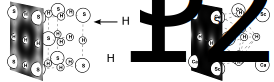
\includegraphics[width=12cm]{Kawamura/charge_ef.pdf}
%       \caption{\label{kawamura_fig_charge_ef}
%         高圧下の硫化水素(左)および新規四元系水素化物(右)の、超伝導に寄与する電子軌道の分布と結晶構造。
%         H、S、Ca、Sc、Yはそれぞれ水素、硫黄、カルシウム、スカンジウム、イットリウム原子を表す。
%         図中の白黒マップは切断面での部分状態密度を表し、明るい部分が大きな値に対応する。}
%     \end{center}
%   \end{figure}

% \begin{招待講演}{1}
\bibitem{kawamura_yitp}
河村光晶,
``超伝導密度汎関数理論の精度検証と応用'',
超伝導研究の発展と広がり,
京都大学基礎物理学研究所,
2023年12月.
\end{招待講演}

\begin{招待論文}{1}
\bibitem{kawamura_kotai}
吉見一慶, 本山裕一, 青山龍美, 川島直輝, 河村光晶,
物性研の計算物性科学コミュニティ支援活動,
固体物理 Vol. 58, No. 9, 29 (2023).
\end{招待論文}

\begin{受賞}{1}
\bibitem{kawamura_hpci1}
HPCIソフトウェア賞【普及部門賞】最優秀賞, 
「計算物質科学ソフトウェア普及活動」, 
MateriAppsチーム (井戸 康太、福田 将大、笠松 秀輔、三澤 貴宏) および PASUMSチーム (本山 裕一, 河村 光晶, 吉見 一慶), 2
023年5月.

\bibitem{kawamura_hpci2}
HPCIソフトウェア賞【開発部門賞】最優秀賞,
「mVMC」, 
mVMC開発チーム (井戸 康太, 森田 悟史, 吉見 一慶, 本山 裕一, 加藤 岳生, 河村 光晶, Ruquing Xu, 今田 正俊, 三澤 貴宏), 
2023年5月.

\bibitem{kawamura_hpci3}
HPCIソフトウェア賞【開発部門賞】優秀賞, 
「$\mathcal{H}\Phi$」, 
$\mathcal{H}\Phi$開発チーム (河村 光晶, 吉見 一慶, 三澤 貴宏, 井戸 康太, 本山 裕一, 山地 洋平), 
2023年5月.
\end{受賞}


\begin{雑誌論文}{4}
\bibitem{kawamura_la2ios2}
H. Ishikawa, T. Yajima, D. Nishio-Hamane, S. Imajo, K. Kindo, and M. Kawamura,
``Superconductivity at 12 K in ${\mathrm{La}}_{2}{\mathrm{IOs}}_{2}$: A $5d$ metal with osmium honeycomb layer'',
Physical Review Materials \textbf{7}, 054804 (2023).

\bibitem{kawamura_hphi}
K. Ido, M. Kawamura, Y. Motoyama, K. Yoshimi, Y. Yamaji, S. Todo, N. Kawashima, T. Misawa,
``Update of $\mathcal{H}\Phi$: Newly added functions and methods in versions 2 and 3'',
Computer Physics Communications \textbf{298}, 109093 (2024).

\bibitem{kawamura_mos2}
F. Ozaki, Dr. S. Tanaka, Y. Choi, W. Osada, K. Mukai, M. Kawamura, M. Fukuda, M. Horio, T. Koitaya, S. Yamamoto, I. Matsuda, T. Ozaki, and J. Yoshinobu,
``Hydrogen-induced Sulfur Vacancies on the $\mathrm{MoS}_2$ Basal Plane Studied by Ambient Pressure XPS and DFT Calculations'',
ChemPhysChem e202300477 (2023).

\bibitem{kawamura_max}
M. Khazaei, S. Bae, R. Khaledialidusti, A. Ranjbar, H. Komsa, S. Khazaei, M. Bagheri, V. Wang, Y. Mochizuki, M. Kawamura, G. Cuniberti, S. M. V. Allaei, K. Ohno, H. Hosono, and H. Raebiger, 
``Superlattice MAX Phases with A-Layers Reconstructed into 0D-Clusters, 1D-Chains, and 2D-Lattices'',
The Journal of Physical Chemistry C \textbf{127}, 30, 14906 (2023).

\end{雑誌論文}



\subsection{野生動物ワイヤレスセンサネットワークと時空間行動分析に関する研究(川瀬 純也)}
本研究室では、野生動物装着型ワイヤレスセンサーネットワーク機構による自然環境下でのデータ収集手法の開発と、それによって得られるデータの解析手法についての研究を行っている。人間が容易には侵入できないエリアでの継続的なデータ収集機構として種々の社会問題の解決に寄与することを目指している。

2023年度は、数年来コロナ禍において中断を余儀なくされていた家畜等の動物による各種実験・データの収集に重点を置いて活動を開始した。協力関係にある企業に依頼し、北海道の広い放牧地で自由に移動し活動する乳牛のGPSデータ等の収集を行った。2箇所の放牧場において、それぞれ6か月・4か月に渡る継続的な放牧牛のGPSデータを収集することができた。これらのGPSデータを用いて、遅延耐性ネットワーク (DTN)技術を用いたワイヤレスセンサーネットワークのシミュレーションを行い、被覆面積の効率的な最大化手法などを検討していく。
 
野生動物を対象に含む時空間行動分析の手法として、配列アライメント手法を用いた類型化手法に着目し、研究を進めている。配列アライメント手法は、もともとはバイオインフォマティクスで用いられる手法であり、編集距離の概念と動的計画法によって、文字列間の類似度を定量的に算出し、類型化する手法である。野生動物の時空間行動は、その意図や目的などを明示的に把握することができず、GPSデータなどの移動データから推測するしかない。そのGPSデータも自然環境下では測位精度が低く、野生動物装着型デバイスのバッテリー持続期間の問題からも、測位の間隔やタイミングが整ったデータを収集することは困難である。多種多様で、大量かつ欠落部分を含む移動データを分析する上で、これらの問題点を考慮した定量的な類型化手法は非常に重要となる。
 
そこで、2023年度に収集した家畜のGPSデータを用いて、これらの類型化手法について検討を進めている。特に、DTN技術を用いた野生動物装着型ワイヤレスセンサーネットワークにおいては、異なる群れの間を行き来したり、積極的に他の個体と接触したりする個体の存在が重要となる。そのような個体が、広くデータを伝播させる役割を担うことができると考えられるからである。類型化手法においては、「一緒に行動する群れ」を特定するだけでなく、「群れの間を行き来するような特徴的な少数派」を効率的に見つけ出すことを目的のひとつとしている。これらの研究成果をまとめ、2024年度中には積極的に報告を進めていく。

% \input{Kawase/ITCannual-list-Kawase}

\subsection{グラフニューラルネットワークとその物性予測問題への応用に関する研究(華井 雅俊)}

% 本節では、2022年度の華井雅俊の研究活動について報告する。グラフニューラルネットワーク(Graph Neural Network, GNN) とその物性予測問題への応用に関する研究に取り組んでいる。
% 電池、半導体、触媒、医薬品などの材料開発・材料研究の全般において、膨大にある候補材料のさまざまな物性を比較解析することが不可欠であるが、それら候補全てを実際に作り検証することは現実的でない。そのため分子構造などの比較的簡単に得られる物質情報から目的の物性を予測・計算することが重要である。近年では、分子構造(グラフ)データとグラフニューラルネットワークを利用した物性値予測モデルの研究が盛んになってきている。2021年度に引き続き、Stanford Universityが取りまとめるOpen Graph Benchmark (OGB) やCMUとFacebookが主導するOpen Catalyst Project (OCP) などの物性予測問題ベンチマークが機械学習系研究コミュニティで取り上げられ、ますますの盛り上がりを見せている。

% 2022年度は、GNNを用いた物理問題へのアプローチに関して大きく2の方向性から取り組んでいる。1つは、既存GNNモデルを物理の問題へ応用した際に現れる機械学習手法の限界に関する研究である。機械学習で典型的な、画像処理や自然言語処理では注力されないが物理の問題では非常に重要となる外挿予測とデータの不均衡性に関して特に取り組んだ~\cite{xsig-limin,xsig-takashige}。
% もう1つは対象の物質により注力した応用研究である。具体的には、ガラスのダイナミクスの予測問題に着手した~\cite{botan}。 ガラスの振る舞いをグラフを用いてモデル化しGNNを用いることで、分子動力学などのシミュレーション結果を詳細に予測した。
% また、その他のGNN応用とも共通の課題として鈴村研究室メンバーとの共同研究も行っており、例えば交通システムの問題に関して研究を行った~\cite{stgtrans}。

% また、業務では情報基盤センターが進めるmdxに関して、物性研究や材料開発で得られるデータの利活用を進めている。本年度は物性データに特化したペタスケールストレージをmdxに連携させるシステムを設計し導入を行った。

% % 一般に、ある物性値が広範囲な材料群に対し既知である場合予測モデルを構築することが可能となるが、しかし一方で、多くの物性値においては既知である材料が少数であり学習データが不足しているため、実用精度の予測モデルを構築することは難しい。同一の物性であってもパラメータや実験条件が共通化されていないと予測モデルの構築は難しいことが知られ、既存の物性予測の研究では、共通の条件で整理された大規模データが主に利用される(例えば、上のコンペティションなど)。小規模に限定されるデータ、例えば計算コストの膨大なシミュレーション値や実験データ、において、機械学習の利用は限定的であり、大きな研究課題の1つとなっている。

% % 我々の研究チームはこのような少規模データに着目し研究を開始した。2021年度下半期は新手法提案への準備としてデータの収集に注力し研究を行った。機械学習分野や材料研究分野で用いられるオープンデータに加え、同学の工学部の研究チームへコンタクトし、スパコンスケールの計算資源を利用し得られた高価なシミュレーション値や実際の実験データに関してヒアリングを行い、データ収集を開始した。
% % また、本部門で開発のすすめるmdxにおいては材料系研究への利用促進を行っており、本研究の中間報告として第20回ナノテクノロジー総合シンポジウムにて発表し、IEEE IC2E 2022への投稿論文にて材料系研究におけるクラウド基盤の利活用をまとめた。

% % % 2021年度は主に、分野の調査と


% % 本節では、2021年度の華井雅俊の研究活動について報告する。2021年9月の本学着任から、グラフニューラルネットワークとその物性予測問題への応用に関する研究に取り組んでいる。

% % 電池、半導体、触媒、医薬品などの材料開発・材料研究の全般において、膨大にある候補材料のさまざまな物性を比較解析することが不可欠であるが、それら候補全てを実際に作り検証することは現実的でない。そのため分子構造などの比較的簡単に得られる物質情報から目的の物性を予測・計算することが重要である。近年では、分子構造(グラフ)データとグラフニューラルネットワークを利用した物性値予測モデルの研究が盛んになってきている。特に2021年度はStanford Universityが取りまとめるOpen Graph Benchmark (OGB) やCMUとFacebookが主導するOpen Catalyst Project (OCP) などの機械学習系研究コミュニティのコンペティションで物性予測問題が取り上げられた初めての年であった。

% % 一般に、ある物性値が広範囲な材料群に対し既知である場合予測モデルを構築することが可能となるが、しかし一方で、多くの物性値においては既知である材料が少数であり学習データが不足しているため、実用精度の予測モデルを構築することは難しい。同一の物性であってもパラメータや実験条件が共通化されていないと予測モデルの構築は難しいことが知られ、既存の物性予測の研究では、共通の条件で整理された大規模データが主に利用される(例えば、上のコンペティションなど)。小規模に限定されるデータ、例えば計算コストの膨大なシミュレーション値や実験データ、において、機械学習の利用は限定的であり、大きな研究課題の1つとなっている。

% % 我々の研究チームはこのような少規模データに着目し研究を開始した。2021年度下半期は新手法提案への準備としてデータの収集に注力し研究を行った。機械学習分野や材料研究分野で用いられるオープンデータに加え、同学の工学部の研究チームへコンタクトし、スパコンスケールの計算資源を利用し得られた高価なシミュレーション値や実際の実験データに関してヒアリングを行い、データ収集を開始した。
% % また、本部門で開発のすすめるmdxにおいては材料系研究への利用促進を行っており、本研究の中間報告として第20回ナノテクノロジー総合シンポジウムにて発表し、IEEE IC2E 2022への投稿論文にて材料系研究におけるクラウド基盤の利活用をまとめた。

% % % 2021年度は主に、分野の調査と




% % \begin{雑誌論文}{1}

% \bibitem{gnn-glass}
% Hayato Shiba, Masatoshi Hanai, Toyotaro Suzumura, and Takashi Shimokawabe, "BOTAN: BOnd TArgeting Network for prediction of slow glassy dynamics by machine learning relative motion." The Journal of Chemical Physics 158, no. 8, 084503, 2022.
% \end{雑誌論文}

% \begin{査読付}{3}

% \bibitem{xsig-limin-hanai}
% Limin Wang, Masatoshi Hanai, Toyotaro Suzumura, Shun Takashige, Kenjiro Taura, "On Data Imbalance in Molecular Property Prediction with Pre-training" xSIG 2023 (submitted)

% \bibitem{xsig-takashige-hanai}
% Shun Takashige, Masatoshi Hanai, Toyotaro Suzumura, Limin Wang, Kenjiro Taura, "Is Self-Supervised Pretraining Good for Extrapolation in Molecular Property Prediction?" xSIG 2023 (submitted)

% \bibitem{stgtrans-xiaohang}
% Xiaohang Xu, Toyotaro Suzumura, Jiawei Yong, Masatoshi Hanai, Chuang Yang, Hiroki Kanezashi, Renhe Jiang, Shintaro Fukushima, "Spatial-Temporal Graph Transformer for Next Point-of-Interest Recommendation", Machine Learning and Knowledge Discovery in Databases: European Conference, (ECML-PKDD), 2023 (submitted)

% \end{査読付}


%\subsection{生態音響システムを用いた生物調査(上坂 怜生)}

% 本節では、2022年度の上坂怜生の研究活動について報告する。本年度は生態音響システムによる高線量地域の鳥類の調査を行った。科学技術振興機構の創発的研究支援事業の一部として行っている本研究では、福島県浪江町の帰宅困難地域内での生態系の経年的変化を音響的手法で調査することを目的としている。当研究室では帰宅困難地域内に設置されたマイクにより過去複数年に渡って調査地の環境音を収集しており、生態学的な価値を持つデータが蓄積され続けている。本年度はこの生態音響データの解析に着手し始めた。実際に福島県浪江町の帰宅困難地域へ赴き、マイクの設置状況等を確認するといった定期的なメンテナンスも行った。本システムによって蓄積されている音響データには特にカラスや鶯といった鳥類の音声が多量に含まれているため、音声の特徴を抽出することでこれら鳥類の出現頻度を検証できるよう解析を進めている。

% また本年度は、生態音響による調査手法を国内のみならず発展途上国の生態系調査へと応用する可能性を鑑み、ネパールの自然保護機関であるNational Trust for Nature Conservation(NTNC)との議論を進めた。福島県の帰宅困難地域という社会的インフラ(電気やインターネット接続)のなかった場所に新たに作り上げた音響システムは、インフラ設備が整っていない発展途上国の広大な野外環境においても応用可能と考えられる。しかし、実現のためには現地の住民や政府機関を含めたステークホルダーの説得や現地研究者の情報技術リテラシー教育など、様々な問題をひとつずつ解決する必要があるため、入念な事前調査が必要である。本年度はネパールのチトワン国立公園を実際に訪れることで、どのような動物がどのような危機にさらされているか事前調査を行った。また、生態音響機材を実際にネパール国内の研究者とともに設置しながら議論を進めることで、生態音響的手法が保全活動に大きく貢献できることを確認した。ネパール国内での調査を福島県浪江町で行っている研究と並行して進めることで、生態音響システムによる生物調査のさらなる発展を促すことができると考えられる。
 
% % \begin{雑誌論文}{1}

% \bibitem{Uesaka2023HCII}
% Uesaka L, Khatiwada AP, Shimotoku D, Parajuli LK, Pandey MR, Kobayashi HH (2023). Applications of Bioacoustics Human Interface System for Wildlife Conservation in Nepal. Accepted for publication in Human Computer Interaction (HCI) International 2023.

% \end{雑誌論文}


\subsection{Research on efficient transformers and mining knowledge from unstructured data(Li Zihui)}

% The first research branch is on efficient transformers. Efficient Transformers are popular for long sequence modeling due to their subquadratic memory and time complexity. However, Sparse Transformer, which improves efficiency by restricting self-attention to predefined sparse patterns, may compromise the expressiveness of the Transformer when important token correlations are distant. To overcome this limitation, we propose Diffuser, an efficient Transformer that incorporates all token interactions within one attention layer while maintaining low computation and memory costs. Diffuser leverages Attention Diffusion to expand the receptive field of sparse attention, allowing it to compute multi-hop token correlations based on all paths between corresponding disconnected tokens. We demonstrate the expressiveness of Diffuser as a universal sequence approximator and its ability to approximate full-attention using a graph expander property. Evaluations show that Diffuser outperforms state-of-the-art benchmarks in both expressiveness and efficiency for language modeling, image modeling, and Long Range Arena (LRA). We also propose a new method that improves the complexity of masked attention from $O(n^2)$ to $O(n)$ by decomposing it into local and global attention. Overall, Diffuser is a promising approach for long sequence modeling that combines the benefits of sparse attention and full-attention. 
% \cite{feng2022diffuser}

% Another research trial proposes a node neighborhood-enhanced framework for knowledge graph completion that enriches the head node information by modeling the head entity neighborhood from multiple hops using graph neural networks. The model also includes an additional edge link prediction task to improve KGC, which is evaluated on two public datasets and demonstrated to be simple yet effective. \cite{li2023nnkgc}

% Lastly, a survey paper reviews the application of deep learning methods for Natural Language Processing (NLP) on electronic health records (EHRs). Recent advances in neural network and deep learning techniques have shown promising results in improving EHR analysis and outperforming traditional statistical and rule-based systems. The survey summarizes various neural NLP methods for EHR applications, including classification, prediction, word embeddings, extraction, generation, question answering, phenotyping, knowledge graphs, medical dialogue, multilinguality, and interpretability. \cite{li2022neural}

% % \begin{雑誌論文}{1}

% \bibitem{sample}
% Irene Li, Jessica Pan, Jeremy Goldwasser, Neha Verma, Wai Pan Wong, Muhammed Yavuz Nuzumlalı, Benjamin Rosand, Yixin Li, Matthew Zhang, David Chang, R. Andrew Taylor, Harlan M. Krumholz, Dragomir Radev,\lq\lq Neural Natural Language Processing for unstructured data in electronic health records: A review", Computer Science Review, volume 46, 2022.

% \end{雑誌論文}

% \begin{査読付}{1}

% \bibitem{feng2022diffuser}
% Aosong Feng and Irene Li and Yuang Jiang andRex  Ying,\lq\lq Diffuser: Efficient Transformers with Multi-hop Attention Diffusion for Long Sequences", Proceedings of Thirty-Seventh AAAI Conference on Artificial Intelligence (AAAI), 2023.

% \end{査読付}

% \begin{発表}{1}

% \bibitem{li2023nnkgc}
% Zihui Li and Boming Yang and Toyotaro Suzumura,\lq\lq NNKGC: Improving Knowledge Graph Completion with Node Neighborhoods", arXiv preprint, 2023.

% \end{発表}

\begin{招待講演}{1}  % invited talks

% sample
% \bibitem{sample-kobayashi3-1}
% Hill Hiroki Kobayashi, mdx: A Cloud Platform for Supporting Data Science and Cross-Disciplinary Research Collaborations, the Nepal JSPS Alumni Association (NJAA), hosted its 7th Symposium, 29 November, 2022.

\bibitem{ireneli-1}
Irene Li, A Journey from Transformers to Large Language Models: an Educational Perspective, 2023 the 1st International Conference on AI-generated Content (AIGC2023), Aug, 2023


\end{招待講演}  % end: invited talks

% \begin{招待論文}{1}  % invited papers



% \end{招待論文}  % end: invited papers


\begin{受賞}{1}  % awards

\bibitem{ireneli-2}
Boming Yang, Dairui Liu, Toyotaro Suzumura, Ruihai Dong and Irene Li,\lq\lq Going Beyond Local: Global Graph-Enhanced Personalized News Recommendations", Proceedings of the 17th ACM Conference on Recommender Systems  (RecSys 2023), 2023 (Best Student Paper Award)

\end{受賞}  % end: awards


% \begin{著書}{1}  % books

% \end{著書}  % end: books


% \begin{雑誌論文}{1}  % journals

% % sample
% % \bibitem{sample-kobayashi1-3}
% % Wenjing Li, Haoran Zhang, Jinyu Chen, Peiran Li, Yuhao Yao, Xiaodan Shi,  Mariko Shibasaki, Hill Hiroki Kobayashi, Xuan Song and Ryosuke Shibasaki, \lq\lq Metagraph-Based Life Pattern Clustering With Big Human Mobility Data", IEEE Transactions on Big Data, Feb, 2023.

% \end{雑誌論文}  % end: journals


\begin{査読付}{1}  % papers (peer-reviewed)

\bibitem{ireneli-3}
Irene Li, Thomas George, Alexander Fabbri, Tammy Liao, Benjamin Chen, Rina Kawamura, Richard Zhou, Vanessa Yan, Swapnil Hingmire and Dragomir Radev, \lq\lq A Transfer Learning Pipeline for Educational Resource Discovery with Application in Leading Paragraph Generation", BEA workshop at Association for Computational Linguistics, 2023

\bibitem{ireneli-4}
Irene Li and Boming Yang, \lq\lq NNKGC: Improving Knowledge Graph Completion with Node Neighborhoods", DL4KG Workshop at International Semantic Web Conference, 2023

\bibitem{ireneli-5}
Linxin Song, Jieyu Zhang, Lechao Cheng, Pengyuan Zhou, Tianyi Zhou and Irene Li, \lq\lq NLPBench: Evaluating Large Language Models on Solving NLP Problems", Instruction Workshop at Conference on Neural Information Processing Systems, 2023


\bibitem{ireneli-6}
Linxin Song, Yan Cui, Ao Luo, Freddy Lecue and Irene Li, \lq\lq Better Explain Transformers by Illuminating Important Information", (Findings) The European Chapter of the Association for Computational Linguistics, 2024

% sample
% \bibitem{sample-kobayashi2-1}
% Daisuk\'e Shimotoku, Tian Yuan, Laxmi Kumar Parajuli and Hill Hiroki Kobayashi,\lq\lq Participatory Sensing Platform Concept for Wildlife Animals in the Himalaya Region, Nepal", Proceedings of 2022 International Conference on Human-Computer Interaction (HCII 2022), 2022.  

\end{査読付}  % end: papers (peer-reviewed)


% \begin{公開}{1}  % open-source urls


% \end{公開}  % end: open-source urls


% \begin{特許}{1}  % patents

% \end{特許}  % end: patents


\begin{発表}{1}  % other talks (Not peer reviewed)

\bibitem{ireneli-7}
Rui Yang, Haoran Liu, Edison Marrese-Taylor, Qingcheng Zeng, Ke Yuhe, Wanxin Li, Lechao Cheng, Qingyu Chen, James Caverlee, Yutaka Matsuo, Irene Li, \lq\lq KG-Rank: Enhancing Large Language Models for Medical QA with Knowledge Graphs and Ranking Techniques", 2024.

\bibitem{ireneli-8}
Hang Jiang, Xiajie Zhang, Robert Mahari, Daniel Kessler, Eric Ma, Tal August, Irene Li, Alex Pentland, Yoon Kim, Jad Kabbara, Deb Roy, \lq\lq Leveraging Large Language Models for Learning Complex Legal Concepts Through Storytelling", 2024.

\bibitem{ireneli-9}
Rui Yang, Boming Yang, Sixun Ouyang, Tianwei She, Aosong Feng, Yuang Jiang, Freddy Lecue, Jinghui Lu, Irene Li, \lq\lq Leveraging Large Language Models for Concept Graph Recovery and Question Answering in NLP Education", 2024.

\bibitem{ireneli-10}
Rui Yang, Qingcheng Zeng, Keen You, Yujie Qiao, Lucas Huang, Chia-Chun Hsieh, Benjamin Rosand, Jeremy Goldwasser, Amisha D Dave, Tiarnan D.L. Keenan, Emily Y Chew, Dragomir Radev, Zhiyong Lu, Hua Xu, Qingyu Chen, Irene Li,\lq\lq Ascle: A Python Natural Language Processing Toolkit for Medical Text Generation", 2024.

\bibitem{ireneli-11}
Fan Gao, Hang Jiang, Rui Yang, Qingcheng Zeng, Jinghui Lu, Moritz Blum, Dairui Liu, Tianwei She, Yuang Jiang, Irene Li, \lq\lq Evaluating Large Language Models on Wikipedia-Style Survey Generation", 2023.

\bibitem{ireneli-12}
Dairui Liu, Boming Yang, Honghui Du, Derek Greene, Aonghus Lawlor, Ruihai Dong, Irene Li, \lq\lq RecPrompt: A Prompt Tuning Framework for News Recommendation Using Large Language Models", 2023.




\end{発表}  % end: other talks (Not peer reviewed)


\begin{報道}{1}  % press (news paper,  televison, etc.)

\bibitem{ireneli-13}
(Interview) Gemma Conroy, \textit{How ChatGPT and other AI tools could disrupt scientific publishing} \footnote{https://www.nature.com/articles/d41586-023-03144-w}, \textbf{Nature, Featured News}, 10 October 2023 

\end{報道}  % end: press (news paper, televison, etc.)



\subsection{生態音響システムを用いた生物調査(上坂 怜生)}

% 本節では、2022年度の上坂怜生の研究活動について報告する。本年度は生態音響システムによる高線量地域の鳥類の調査を行った。科学技術振興機構の創発的研究支援事業の一部として行っている本研究では、福島県浪江町の帰宅困難地域内での生態系の経年的変化を音響的手法で調査することを目的としている。当研究室では帰宅困難地域内に設置されたマイクにより過去複数年に渡って調査地の環境音を収集しており、生態学的な価値を持つデータが蓄積され続けている。本年度はこの生態音響データの解析に着手し始めた。実際に福島県浪江町の帰宅困難地域へ赴き、マイクの設置状況等を確認するといった定期的なメンテナンスも行った。本システムによって蓄積されている音響データには特にカラスや鶯といった鳥類の音声が多量に含まれているため、音声の特徴を抽出することでこれら鳥類の出現頻度を検証できるよう解析を進めている。

% また本年度は、生態音響による調査手法を国内のみならず発展途上国の生態系調査へと応用する可能性を鑑み、ネパールの自然保護機関であるNational Trust for Nature Conservation(NTNC)との議論を進めた。福島県の帰宅困難地域という社会的インフラ(電気やインターネット接続)のなかった場所に新たに作り上げた音響システムは、インフラ設備が整っていない発展途上国の広大な野外環境においても応用可能と考えられる。しかし、実現のためには現地の住民や政府機関を含めたステークホルダーの説得や現地研究者の情報技術リテラシー教育など、様々な問題をひとつずつ解決する必要があるため、入念な事前調査が必要である。本年度はネパールのチトワン国立公園を実際に訪れることで、どのような動物がどのような危機にさらされているか事前調査を行った。また、生態音響機材を実際にネパール国内の研究者とともに設置しながら議論を進めることで、生態音響的手法が保全活動に大きく貢献できることを確認した。ネパール国内での調査を福島県浪江町で行っている研究と並行して進めることで、生態音響システムによる生物調査のさらなる発展を促すことができると考えられる。
 
% % \begin{雑誌論文}{1}

% \bibitem{Uesaka2023HCII}
% Uesaka L, Khatiwada AP, Shimotoku D, Parajuli LK, Pandey MR, Kobayashi HH (2023). Applications of Bioacoustics Human Interface System for Wildlife Conservation in Nepal. Accepted for publication in Human Computer Interaction (HCI) International 2023.

% \end{雑誌論文}


% Ishikawa group
\subsection{高速知能システムの研究(石川正俊)}

%  本研究室では、センサ情報処理における並列処理を基盤として、高速・リアルタイム性を有するセンサ情報処理を高度に実現し、高速知能システムとして実装する研究を行っている。具体的には、以下4つの分野での研究開発を行っている。また、各分野での新規産業開拓にも力を注ぎ、研究成果の技術移転、共同研究、事業化等を様々な形で積極的に推進している。

% センサフュージョンの研究では、高速のセンサフィードバックに関する理論並びにシステムアーキテクチャの構築、その高速知能ロボットとしての実装、並びに高速性を活かした新規タスクの実現、特に、センサ情報に基づく人間機械協調システムの開発を行っている。

% ダイナミックビジョンシステムの研究では、高速ビジョンや動的光学系に基づき運動対象の情報を適応的に取得する基礎技術の開発、特に、高速光軸制御や適応光学系の技術開発やトラッキング撮像に関する応用システムの開発を行っている。

% システムビジョンデザインの研究では、高速三次元形状計測や高速質感計測など、並列処理に基づく高速画像処理技術 (理論、アルゴリズム、デバイス) の開発とその応用システムの実現を目指し、特に高速画像処理システムの開発や応用システムの開発を行っている。

% アクティブパーセプションの研究では、実世界における新たな知覚補助技術並びにそれに基づく新しい対話の形の創出を目指し、特に各種高速化技術を用いた能動計測や能動認識を利用した革新的情報環境・ヒューマンインタフェイスの開発を行っている。

% これらの研究では、原則的に並列かつリアルタイムの演算構造を有する現実の物理世界と同等の構造を工学的に実現することを目指しており、そのことにより、現実世界の理解を促すばかりでなく、従来のシステムをはるかに凌駕する性能を有する高速知能システムを生み出すことができ、結果として、まったく新しい情報システムを構築することが可能となる。


%% \begin{雑誌論文}{1}
% \bibitem{01石川正俊01}
% Masatoshi Ishikawa, Idaku Ishii, Hiromasa Oku, Akio Namiki, Yuji Yamakawa, and Tomohiko Hayakawa: Special Issue on High-Speed Vision and its Applications, Journal of Robotics and Mechatronics, Vol.34, No.5, p.911, 2022.

% \bibitem{01石川正俊02}
% Taku Senoo, Atsushi Konno, Yunzhuo Wang, Masahiro Hirano, Norimasa Kishi, and Masatoshi Ishikawa: Tracking of Overlapped Vehicles with Spatio-Temporal Shared Filter for High-Speed Stereo Vision, Journal of Robotics and Mechatronics, Vol.34, No.5, pp.1033-1042, 2022.

% \bibitem{01石川正俊03}
% Hyuno Kim, Yuji Yamakawa, and Masatoshi Ishikawa: Seamless Multiple-Target Tracking Method Across Overlapped Multiple Camera Views Using High-Speed Image Capture, Journal of Robotics and Mechatronics, Vol.34, No.5, pp.1043-1052, 2022.

% \bibitem{01石川正俊04}
% Masatoshi Ishikawa: High-Speed Vision and its Applications Toward High-Speed Intelligent Systems, Journal of Robotics and Mechatronics, Vol.34, No.5, pp.912-935 , 2022.

% \end{雑誌論文}

% \begin{発表}{1}

% \bibitem{01石川正俊05}
% Taku Senoo, Atsushi Konno, Yunzhuo Wang, Masahiro Hirano, Norimasa Kishi, and Masatoshi Ishikawa: Automotive Tracking with High-speed Stereo Vision Based on a Spatiotemporal Shared Filter, the 2022 26th International Conference on System Theory, Control and Computing (ICSTCC2022), Proceedings, pp.613-618, 2022.

% \end{発表}

% \begin{報道}{1}

% \bibitem{01石川正俊06}
% 石川グループ研究室: 世界!オモシロ学者のスゴ動画祭3, NHK, 2022年7月8日, BSプレミアム

% \end{報道}

%\subsection{革新的情報環境構築に向けた能動計測型高速トラッキングシステムの研究開発(早川智彦)}

%  2022年度は主に高速画像処理を用いた高速トラッキングシステムの開発を実施し、主に1.白線認識を用いた高速道路における高速撮像システムの研究、2.高速画角切り替えによる画角拡張システムの開発を実施した。全体を通した研究成果として、2件の雑誌論文(査読付)、1件の解説論文、3件の査読付き国際学会予稿と1件の雑誌以外の査読なし国内学会予稿に採択された。

% 1.白線認識を用いた高速道路における高速撮像システムの研究
% 高速道路のトンネルにおける自己位置推定手法として、GPSでは電波を捕捉できないため機能せず、加速度センサでは十分な精度が得られないため、白線認識を利用した自己位置推定手法を開発した。この手法では、白線を画像で撮像することで、その見え方から自己位置を推定することが可能であり、自己位置を元に、トンネル天井面の撮像角度を任意の角度へと補償しながら撮像し続けることが可能となる。これにより、運転手の技量に頼ることなく、狙った位置を撮像し続けることができ、点検の効率向上に寄与する技術といえる。この成果を国際論文誌に投稿し、採択に至った。また、インフラ点検の関連技術をまとめ、関連技術を解説論文にも投稿することで、技術の社会実装が円滑に進むよう努めた。

% 2.高速画角切り替えによる画角拡張システムの開発
% 画角と解像度はトレードオフの関係にあるが、画角をミラーによって高速に切り替えることで、仮想的に画角の拡張を実現する技術を開発した。これにより、例えば高速道路の点検といった応用において、高解像度な画像を少ないカメラ台数で複数回に渡り撮像する状況において、その撮像回数を大幅に減少させることが可能となる。この成果を国際論文誌に投稿し、採択に至った。

\subsection{アクティブパーセプションとその応用展開(早川智彦)}

2023年度は主に1.高速画像処理技術による点検の高度化、2.光学的能動マーカーによるトラッキング技術の開発、3.人間の視線情報のトラッキングによる情報提示手法の開発を実施した。全体を通した研究成果として、1件の雑誌論文(査読付)、5件の雑誌以外の査読付き論文、2件の招待講演、2件の査読なしの発表を行った。

 1.高速画像処理技術による点検の高度化
インフラ点検において正確に点検対象の位置を捕捉するため、車両の自己位置の把握は必須となる。そこで、本研究ではトンネルに存在する照明装置の位置を認識することで、車両から追加の照明やレーザー照射を利用すること無く、正確に車両の自己位置を求める手法を開発し、実際に高速道路上で試すに至った。結果として、狙った位置にある特定のひび割れを時速100kmで走行しながら高分解撮像することができた。本内容を元に、論文投稿1件や国際学会発表2件、国内学会発表2件の成果を得られた。

 2.光学的能動マーカーによるトラッキング技術の開発
マーカーを用いずに動的対象をトラッキングするため、レーザー加温と紫外線照射による蓄光によって、高速にマーカーを生じさせる手法を開発し、国際学会にて発表を行った。どちらの手法もトラッキングに対して有用であることを明らかにしたため、今後それぞれの手法に適した状況にあわせて使い分けられる予定である。本成果で招待講演1件と国際学会の発表2件を行った。

 3.人間の視線情報のトラッキングによる情報提示手法の開発
人の視線情報にあわせてフレームレートを可変とすることで、人の知覚情報量を変えること無く計算機の計算量を低減させる手法を開発した。実験によって原理の検証を行い、国際学会にて発表した。

%\begin{招待講演}{1}
\bibitem{01早川智彦01}
Tomohiko Hayakawa:  User Performance based on the Effects of Low Video Latency between Visual and Haptic Information in Immersive Environments (Invited), The 6th International Conference on Intelligent Robotics and Control Engineering (IRCE 2023), 2023.8

\bibitem{01早川智彦02}
Tomohiko Hayakawa:  Optical axis control methods for infrastructure inspection, 2nd Intl. Conference Advances in 3OM , OPT23-42,Timisoara, 2023.12

\end{招待講演}

\begin{査読付}{1}

\bibitem{01早川智彦03}
Yushi Moko, Yuka Hiruma, Tomohiko Hayakawak, Yuriko Ezaki, Yoshimasa Onishi, Masatoshi Ishikawa:A method for calculating crack width using chalking marks in low-contrast 2D images acquired during high-speed driving, In Proc. Of SPIE 12952, 4,2024.3

\bibitem{01早川智彦04}
Tomohiko Hayakawak, Yuka Hiruma, Ke Yushan, Masatoshi Ishikawa
Label-free position tracking in stuffed sparrow using phosphorescence, Conf. on Label-free Biomedical Imaging and Sensing (LBIS) 2024, SPIE Photonics West BiOS, San Francisco,2024.1

\bibitem{01早川智彦05}
Yuki Kubota, Tomohiko Hayakawa, and Masatoshi Ishikawa: Visual Search Tasks under Spatio-Temporal Control Synchronized with Eye Movements, In Proceedings of the 2023 Symposium on Eye Tracking Research and Applications (ETRA '23), Association for Computing Machinery, Article 43, pp.1-2,New York, USA, 2023.6

\bibitem{01早川智彦06}
Yushi Moko, Yuka Hiruma, Tomohiko Hayakawak, Yoshimasa Onishi, Masatoshi Ishikawa:  High-Speed Localization Estimation Method Using Lighting Recognition in Tunnels, 2023 7th International Conference on Intelligent Traffic and Transportation(ICITT 2023) , ML755,Madrid,2023.9

\bibitem{01早川智彦07}
Tomohiko Hayakawa, Yuka Hiruma, Yushan Ke, Masatoshi Ishikawa: Active thermal marker using thermal images of heated areas with visible semiconductor laser, the 10th edition of the International Conference on Optical and Photonic Engineering(icOPEN 2023), 15617, Singapore, 2023.11

\end{査読付}

\begin{発表}{1}

\bibitem{01早川智彦08}
望戸雄史,早川智彦,大西偉允,石川正俊:  トンネル内における照明認識による自己位置推定手法,令和5年度土木学会全国大会第78回学術講演会, CS9-24, 広島, 2023.9

\bibitem{01早川智彦09}
望戸雄史, 蛭間友香, 早川智彦, 柯毓珊, 大西偉允, 石川正俊:  照明認識を利用した高速道路のトンネル外観検査のための自己位置推定手法, 第21回ITSシンポジウム2023, 2-B-13, 富山, 2023.12

\end{発表}



\subsection{知能ロボットおよび人間機械協調の実現に向けた研究開発(黄守仁)}

%  本年度は主に生産システムの知能化を目指した動的補償ロボットの開発と評価実験、無拘束の視線入力などに基づく人間・ロボットの協調の提案および実装、高速三次元計測によるロボット制御などの研究内容で研究活動を行った。

% 生産システムの知能化を目指した(企業との)共同研究において、前年度の研究を継続し、一般的な産業用ロボットが速度・精度・不確定要素に対する適応能力の三者を同時に成立させることが難しい現状に対して、高帯域でのセンシング・動作によるローカル誤差吸収と低い帯域でのグローバル計画動作を並列に行う動的補償手法を提案し、コンベア上を流れている事前情報(置く位置・姿勢、塗布形状などの情報を指す)のない部品に対する高精度な塗布作業の実現を可能とするロボットを開発した。初期の評価実験で得られた結果を計測自動制御学会システムインテグレーション部門SI2022にて発表を行い、研究成果が認められ、優秀講演賞を受賞した。

% 次に、次世代サイボーグシステムの実現に向けて、無拘束の視線入力とロボットによるセンシング支援・動作支援を統合する人間機械協調手法を提案し、ROS環境での実装および予備実験を行った。室内の日常生活を想定し、人間の視線入力とロボットの視覚センシング支援および動作支援の応用場面を検討した。特に、南デンマーク大学からの博士課程学生が協力研究補助員として短期訪問をしている間、システム実装に向けてとても有意義な交流を行った。

% また、企業との共同研究課題として、高速三次元計測を動的補償ロボット制御に統合するシステムの設計およびシミュレーションモデル構築など、前年度の研究活動も継続して取り組んでいる。

%% \begin{受賞}{1}

% \bibitem{03黄守仁01}
% 黄守仁,村上健一, 石川正俊: 対象の事前情報必要としない動的塗布応用に向けたロボットの実現, 第23回計測自動制御学会システムインテグレーション部門講演会(SI2022), 講演会論文集, pp.999-1001, SI2022 優秀講演賞, 2022.

% \end{受賞}

% \begin{雑誌論文}{1}

% \bibitem{03黄守仁02}
% Kenichi Murakami, Shouren Huang, Masatoshi Ishikawa, and Yuji Yamakawa: Fully Automated Bead Art Assembly for Smart Manufacturing Using Dynamic Compensation Approach, J. Robot. Mechatron., Vol.34, No.5, pp.936-945, 2022. 

% \bibitem{03黄守仁03}
% Shouren Huang, Kenichi Murakami, Masatoshi Ishikawa, Yuji Yamakawa: Robotic Assistance Realizing Peg-and-Hole Alignment by Mimicking the Process of an Annular Solar Eclipse, Journal of Robotics and Mechatronics, Vol.34 No.5, pp.946-955, 2022. 

% \end{雑誌論文}

% \begin{発表}{1}

% \bibitem{03黄守仁04}
% 黄守仁, 村上健一, 石川正俊: 対象の事前情報必要としない動的塗布応用に向けたロボットの実現, 第23回計測自動制御学会システムインテグレーション部門講演会(SI2022), 講演会論文集, pp.999-1001, 2022.

% \bibitem{03黄守仁05}
% 村上健一,黄守仁,石川正俊,山川雄司: 動的補償を用いたビーズピッキング, 第40回日本ロボット学会学術講演会 (RSJ2022), 予稿集, 4C1-05, 2022.

% \bibitem{03黄守仁06}
% Shouren Huang, Yongpeng Cao, Kenichi Murakami, Masatoshi Ishikawa,Yuji Yamakawa: Bimanual Coordination Protocol for the Inter-Limb Transmission of Force Feedback, 第40回日本ロボット学会学術講演会 (RSJ2022), 予稿集, 2C1-05, 2022.

% \end{発表}


\subsection{ダイナミックビジョンシステムとその応用展開(末石智大)}

 高速画像処理および高速光学系制御を活用する、動的検査技術とヒューマンインターフェースに関するダイナミックビジョンシステムの研究を実施した。

実世界の動的かつ複雑な現象を適応的にデータ化し、意味のある形で活用する動的検査技術として,本年度もマイクロサッカードと呼ばれる眼球微振動を対象として実施した。頭部固定を必要としない計測条件でのマイクロサッカード検出は、被験者を拘束する負荷や時間効率の観点から高い有効性が期待される。リラックスした状態の人間のマイクロサッカード検出に向けて、回転ミラーや液体可変焦点レンズなどの光学素子を高速に制御しつつ高解像度合焦画像計測を達成することで、ダイナミックビジョンシステムにおける動的検査への基礎技術の研鑽を本年度も進めている。本技術の定量的評価のための動的眼球模型の両眼化など、周辺技術の開発による成果も実現している。

また、昨年度に引き続き球技スポーツであるテニスのライン判定を目的とした高速ビジョンと落下位置予測技術の融合システムの研究も進めており、本年度は国際学会においても受賞を獲得した。高速なカルマンフィルタに基づくテニスボールの落下予測位置に対して先行した光学系制御による、地面テクスチャの高解像度撮影を実現することで、比較的単純な差分処理によりボール着地痕跡を可視化する技術である。
ヒューマンインターフェースに関しては、ボールの高速落下位置予測を活用した、ダイナミックプロジェクションマッピングによる先読み情報提示や、円筒鏡面と即時フィードバックを活用した視点依存ディスプレイの一種であるダイナミックアナモルフォーシスシステムも実現している。特に後者のアナモルフォーシスシステムは、国内学会における優秀講演賞も獲得している。

本年度は総じて、運動予測も包含させた高速センシング技術を洗練し、検査やダイナミックプロジェクションマッピングへの実世界応用の展開を成熟させた。

%% \begin{受賞}{1}

% \bibitem{04末石智大01}
% 栃岡陽麻里, 末石智大, 石川正俊: 球技スポーツの着地痕跡判定に向けた高速ビジョンを用いた落下位置予測, 第23回計測自動制御学会システムインテグレーション部門講演会(SI2022), 講演会論文集, pp.2089-2092, 優秀講演賞, 2022.

% \end{受賞}

% \begin{雑誌論文}{1}

% \bibitem{04末石智大02}
% 井上満晶, 末石智大, 松村蒼一郎, 谷内田尚司, 細井利憲, 石川正俊: 非接触マイクロサッカード検出に向けた高速追跡を用いた眼球運動検出システム, 生体医工学, Vol. 60, No. 6, pp.170-174, 2022.

% \bibitem{04末石智大03}
% Tomohiro Sueishi, Ryota Nishizono, and Masatoshi Ishikawa: EmnDash:A Robust High-Speed Spatial Tracking System Using a Vector-Graphics Laser Display with M-Sequence Dashed Markers, J. Robot. Mechatron., Vol.34, No.5, pp.1085-1095, 2022.

% \end{雑誌論文}

% \begin{発表}{1}

% \bibitem{04末石智大04}
% 末石智大, 井上満晶, 谷内田尚司, 石川正俊: 照明制御に基づく動的眼球高速トラッキングによる明瞳孔微振動画像計測, 動的画像処理実利用化ワークショップ2023(DIA2023), 講演論文集, pp.133-136, IS1-20, 2023.

% \bibitem{04末石智大05}
% 栃岡陽麻里, 末石智大, 石川正俊: 球技スポーツの着地痕跡判定に向けた高速ビジョンを用いた落下位置予測, 第23回計測自動制御学会システムインテグレーション部門講演会(SI2022), 講演会論文集, pp.2089-2092, 2022.

% \bibitem{04末石智大06}
% 末石智大, 石川正俊: 縞状同心円パターンを用いた可変焦点制御系のカメラ校正手法, 第23回計測自動制御学会システムインテグレーション部門講演会(SI2022), 講演会論文集, pp.2093-2097, 2022.

% \bibitem{04末石智大07}
% 井上満晶, 末石智大, 松村蒼一郎, 谷内田尚司, 細井利憲, 石川正俊: 非接触マイクロサッカード検出に向けた高速追跡を用いた眼球運動検出システム, 生体医工学シンポジウム2022(オンライン), 予稿・抄録集, p.13, 1A-11, 2022.

% \bibitem{04末石智大08}
% 末石智大, 石川正俊: 高速光学系制御と対称的ドットマーカによる卓球回転実時間計測, 第40回日本ロボット学会学術講演会 (RSJ2022), 予稿集, 2B1-08, 2022.

% \end{発表}


\subsection{高速3次元形状計測技術の評価と応用(宮下令央)}

%  本年度は昨年度開発した高速3次元形状計測技術の評価、および関連する高速画像処理システムの研究・発表を行った。
%  新たに開発した高速3次元形状計測技術によって、従来手法よりも高解像度かつ高精度な3次元形状計測が1,000fpsを超える高速性と低遅延性を維持したまま実現できることを確認し、成果を国内外で発表した。

% また、高速3次元形状計測の関連研究として、従来のテレセントリック光学系による画像検査では困難な長尺の棒材の寸法検測を非テレセントリック光学系によって実現するシステムや、高速3次元形状計測と高速法線計測を統合して高密度かつ高精度かつ高速な3次元形状計測を実現するシステム、さらにイメージセンサに高速画像処理を行うプロセッサを並置したビジョンチップを用いて小型化を実現した高速光軸制御システムについて、論文誌において発表を行った。

% さらに、人間の錯覚を利用して仮想的な運動を付加するダイナミックプロジェクションマッピング技術をコンピュータグラフィックスに応用し、アニメーションのレンダリングを高速化する研究を行い、被験者実験を通して得た人間の知覚特性に関する知見について国際学会において発表を行った。
% 今後は高速3次元形状計測技術を発展させ、質感計測やダイナミックプロジェクションマッピングへの応用を進めていく予定である。

% また、解説論文の執筆、研究会の運営や査読を通して学会への貢献を続けている。

%% \begin{招待論文}{1}

% \bibitem{05宮下令央01}
% 宮下 令央, 末石 智大, 田畑 智志, 早川 智彦, 石川 正俊: 高速ビジョンが拓くダイナミックプロジェクションマッピング技術, 電子情報通信学会 通信ソサイエティマガジン B-plus, 解説論文, No.64, pp.275-284, 2023. 

% \end{招待論文}

% \begin{雑誌論文}{1}

% \bibitem{05宮下令央02}
% Leo Miyashita, Masatoshi Ishikawa: Portable High-speed Optical Gaze Controller with Vision Chip, Journal of Robotics and Mechatronics(JRM), Vol.34, No.5, pp.1133-1140, 2022.

% \bibitem{05宮下令央03}
% Leo Miyashita, Yohta Kimura, Satoshi Tabata, Masatoshi Ishikawa: High-speed Depth-normal Measurement and Fusion Based on Multiband Sensing and Block Parallelization, Journal of Robotics and Mechatronics (JRM), Vol.34, No.5, pp.1111-1121, 2022.

% \bibitem{05宮下令央04}
% Leo Miyashita, Masatoshi Ishikawa: Real-Time Inspection of Rod Straightness and Appearance by Non-Telecentric Camera Array, Journal of Robotics and Mechatronics (JRM), Vol.34, No.5, pp.975-984, 2022.

% \bibitem{05宮下令央05}
% Yunpu Hu, Leo Miyashita, and Masatoshi Ishikawa: Differential Frequency Heterodyne Time-of-Flight Imaging for Instantaneous Depth and Velocity Estimation. ACM Trans. Graph. Vol.42, No.1, Article 9, pp.9, 2022.

% \end{雑誌論文}

% \begin{査読付}{1}

% \bibitem{05宮下令央06}
% 宮下 令央, 田畑 智志, 石川 正俊: パラレルバスパターンによる高速低遅延3次元形状計測, 計測自動制御学会, 第39回 センシングフォーラム, 1B1-1, 予稿集 pp.49-54, 2022.

% \bibitem{05宮下令央07}
% Leo Miyashita, Satoshi Tabata, Masatoshi Ishikawa: High-speed and Low-latency 3D Sensing with a Parallel-bus Pattern, International Conference on 3D Vision(3DV2022), 2022.

% \bibitem{05宮下令央08}
% Leo Miyashita, Kentaro Fukamizu, Yuki Kubota, Tomohiko Hayakawa, Masatoshi Ishikawa: Real-time animation display based on optical illusion by overlaid luminance changes, SPIE Optical Architectures for Displays and Sensing in Augmented, Virtual, and Mixed Reality(AR, VR, MR)IV, Oral, paper 12449-8, 2023.

% \end{査読付}


% \subsection{小型高速三次元スキャナの開発および可変光学系による技術拡張に関する研究(田畑智志)}

%  本年度は主に小型高速三次元スキャナの開発を昨年度に引き続き実施するとともに、計測システムの可変焦点化による計測技術の向上方法の検討と、形状計測の高精度高解像化やダイナミックプロジェクションマッピング技術の広範囲化に関する実験を実施した。

% 高速三次元スキャン技術は、運動する物体の形状取得やロボットにおける外界認識・インタラクションなど、高速性・リアルタイム性が要求される応用において重要である。昨年度に引き続き、小型ユニットを用いた1,000fpsでの高速小型三次元スキャナの開発を行い、国内学会での口頭発表や招待論文、報道による周知を行った。
% リアルタイムのモデル生成と運動補正を組みあわせることで1,000fpsの高速性を維持したまま、1辺10cmの立方体に収まるサイズで片手に持ってスキャン可能な計測システムを実現している。また、この技術をさらに発展させるため、さらなる統合アプローチの検討を進めている。

% さらに、三次元形状計測について、計測距離範囲・精度を向上させるため高速可変焦点レンズの導入を進め予備実験を実施した。また、位相シフト法における計測精度の向上や高解像化に際して課題となる点を精査し、それぞれの課題を解決するためのアルゴリズムの開発を進めている。

% また、ダイナミックプロジェクションマッピングに関しては、対象の三次元的な情報を計測・利用するシステムに対する回転ミラーを用いたトラッキングアプローチの拡張を進めており、実際の応用を通じた実験を行っている。



%% \begin{招待論文}{1}

% \bibitem{06田畑智志01}
% 田畑智志, 渡辺義浩, 石川正俊: 小型高速三次元スキャナの研究開発と将来展望, 日本ロボット工業会機関紙『ロボット』, 271号, pp.45-47, 2023.

% \end{招待論文}

% \begin{雑誌論文}{1}

% \bibitem{06田畑智志02}
% Lihui Wang, Satoshi Tabata, Hongjin Xu, Yunpu Hu, Yoshihiro Watanabe, and Masatoshi Ishikawa: Dynamic depth-of-field projection mapping method based on a variable focus lens and visual feedback, Optics Express, Vol.31, Issue 3, pp.3945-3953, 2023.

% \bibitem{06田畑智志03}
% Hao Xu, Satoshi Tabata, Haowen Liang, Lihui Wang, and Masatoshi Ishikawa: Accurate measurement of virtual image distance for near-eye displays based on auto-focusing, Applied Optics, Vol.61, Issue 30, pp.9093-9098, 2022.

% \bibitem{06田畑智志04}
% Yuping Wang, Senwei Xie, Lihui Wang, Hongjin Xu, Satoshi Tabata, and Masatoshi Ishikawa, ARSlice: Head-Mounted Display Augmented with Dynamic Tracking and Projection, Journal of Computer Science and Technology, Vol.37, Issue 3, pp.666-679, 2022.

% \end{雑誌論文}

% \begin{査読付}{1}

% \bibitem{06田畑智志05}
% Yuping Wang, Senwei Xie, Lihui Wang, Hongjin Xu, Satoshi Tabata, Masatoshi Ishikawa: Head-Mounted Display Augmented with Dynamic Tracking and Projection, The 10th international conference on Computational Visual Media(CVM 2022), 2022.

% \end{査読付}

% \begin{発表}{1}

% \bibitem{06田畑智志06}
% 田畑智志, 渡辺義浩, 石川正俊: 小型高速三次元スキャナの開発, 第40回日本ロボット学会学術講演会(RSJ2022), 予稿集, 2B1-07, 2022.

% \end{発表}

% \begin{報道}{1}

% \bibitem{06田畑智志07}
% 田畑智志: 毎秒1000回撮像で立体計測 小型高速3Dスキャナー ロボアームの高速操作向け 東大など開発, 日刊工業新聞, 2022年9月27日.

% \end{報道}



\section{データ科学研究部門 成果要覧}
\begin{招待講演}{1}

\bibitem{01早川智彦01}
Tomohiko Hayakawa:  User Performance based on the Effects of Low Video Latency between Visual and Haptic Information in Immersive Environments (Invited), The 6th International Conference on Intelligent Robotics and Control Engineering (IRCE 2023), 2023.8

\bibitem{01早川智彦02}
Tomohiko Hayakawa:  Optical axis control methods for infrastructure inspection, 2nd Intl. Conference Advances in 3OM , OPT23-42,Timisoara, 2023.12


\bibitem{02末石智大01}
末石智大: 高速光学系制御による動的イメージングシステムとその応用, 高速度イメージングとフォトニクスに関する総合シンポジウム2023, 近畿大学, 大阪, 2023.12


\bibitem{hanai-simpo}
華井雅俊、
"ARIM-mdxデータシステム",
ARIM「第2回革新的なエネルギー変換を可能とするマテリアル領域」シンポジウム,
2024年1月

\bibitem{hanai-utac}
華井雅俊,
"ARIM-mdxデータシステム: 材料実験データの利活用に向けた実験施設のDX化", 
第一回UDAC-SRIS合同勉強会,
2023年12月

\bibitem{hanai-gizyutsu}
華井雅俊、
"ARIM-mdxデータシステム"
ARIM 第1回計測技術スタッフ全体研修会,
2023年12月

\bibitem{kawamura_yitp}
河村光晶,
``超伝導密度汎関数理論の精度検証と応用'',
超伝導研究の発展と広がり,
京都大学基礎物理学研究所,
2023年12月.
\bibitem{ykuga45871732}
空閑洋平, データセンタハードウェアへのソフトウェア脆弱試験の適応, Society 5.0時代の安心・安全・信頼を支える基盤ソフトウェア技術の構築, 2024年3月.


\bibitem{ireneli-1}
Irene Li, A Journey from Transformers to Large Language Models: an Educational Perspective, 2023 the 1st International Conference on AI-generated Content (AIGC2023), Aug, 2023


\end{招待講演}

\begin{招待論文}{1}

\bibitem{kawamura_kotai}
吉見一慶, 本山裕一, 青山龍美, 川島直輝, 河村光晶,
物性研の計算物性科学コミュニティ支援活動,
固体物理 Vol. 58, No. 9, 29 (2023).
\bibitem{ykuga45871752}
河原大輔, 空閑洋平, 黒橋禎夫, 鈴木潤, 宮尾祐介, LLM-jp: 日本語に強い大規模言語モデルの研究開発を行う組織横断プロジェクト, 自然言語処理, 31, 1, pp266-279, 2024年.

\end{招待論文}

\begin{受賞}{1}

\bibitem{02末石智大02}
Himari Tochioka, Tomohiro Sueishi, and Masatoshi Ishikawa: SICE Annual Conference International Award, SICE Annual Conference 2023,2023.9

\bibitem{02末石智大03}
田畑智志,末石智大,宮下令央,石川正俊: 2023年 計測自動制御学会 システムインテグレーション部門SI2023 優秀講演賞,第24回計測自動制御学会システムインテグレーション部門講演会 (SI2023), 新潟,2023.12

\bibitem{kawamura_hpci1}
HPCIソフトウェア賞【普及部門賞】最優秀賞, 
「計算物質科学ソフトウェア普及活動」, 
MateriAppsチーム (井戸 康太、福田 将大、笠松 秀輔、三澤 貴宏) および PASUMSチーム (本山 裕一, 河村 光晶, 吉見 一慶), 2
023年5月.

\bibitem{kawamura_hpci2}
HPCIソフトウェア賞【開発部門賞】最優秀賞,
「mVMC」, 
mVMC開発チーム (井戸 康太, 森田 悟史, 吉見 一慶, 本山 裕一, 加藤 岳生, 河村 光晶, Ruquing Xu, 今田 正俊, 三澤 貴宏), 
2023年5月.

\bibitem{kawamura_hpci3}
HPCIソフトウェア賞【開発部門賞】優秀賞, 
「$\mathcal{H}\Phi$」, 
$\mathcal{H}\Phi$開発チーム (河村 光晶, 吉見 一慶, 三澤 貴宏, 井戸 康太, 本山 裕一, 山地 洋平), 
2023年5月.
\bibitem{ykuga43010880}
空閑洋平, 山下記念研究賞, 情報処理学会(OS研究会), 2024年3月.

\bibitem{ykuga43010877}
空閑洋平, 山下記念研究賞, 情報処理学会(IOT研究会), 2024年3月.

\bibitem{ykuga43010874}
空閑洋平, 中村遼, 藤村記念ベストプラクティス賞, 情報処理学会(IOT研究会), 2023年7月.

\bibitem{ykuga9999}
中村遼, 空閑洋平, 明石邦夫, Most Innovative for HPC Uses Award, Data Mover Challenge 2023, 2024年2月.


\bibitem{ireneli-2}
Boming Yang, Dairui Liu, Toyotaro Suzumura, Ruihai Dong and Irene Li,\lq\lq Going Beyond Local: Global Graph-Enhanced Personalized News Recommendations", Proceedings of the 17th ACM Conference on Recommender Systems  (RecSys 2023), 2023 (Best Student Paper Award)

\end{受賞}

\begin{著書}{1}

\end{著書}

\begin{雑誌論文}{1}

\bibitem{kawamura_la2ios2}
H. Ishikawa, T. Yajima, D. Nishio-Hamane, S. Imajo, K. Kindo, and M. Kawamura,
``Superconductivity at 12 K in ${\mathrm{La}}_{2}{\mathrm{IOs}}_{2}$: A $5d$ metal with osmium honeycomb layer'',
Physical Review Materials \textbf{7}, 054804 (2023).

\bibitem{kawamura_hphi}
K. Ido, M. Kawamura, Y. Motoyama, K. Yoshimi, Y. Yamaji, S. Todo, N. Kawashima, T. Misawa,
``Update of $\mathcal{H}\Phi$: Newly added functions and methods in versions 2 and 3'',
Computer Physics Communications \textbf{298}, 109093 (2024).

\bibitem{kawamura_mos2}
F. Ozaki, Dr. S. Tanaka, Y. Choi, W. Osada, K. Mukai, M. Kawamura, M. Fukuda, M. Horio, T. Koitaya, S. Yamamoto, I. Matsuda, T. Ozaki, and J. Yoshinobu,
``Hydrogen-induced Sulfur Vacancies on the $\mathrm{MoS}_2$ Basal Plane Studied by Ambient Pressure XPS and DFT Calculations'',
ChemPhysChem e202300477 (2023).

\bibitem{kawamura_max}
M. Khazaei, S. Bae, R. Khaledialidusti, A. Ranjbar, H. Komsa, S. Khazaei, M. Bagheri, V. Wang, Y. Mochizuki, M. Kawamura, G. Cuniberti, S. M. V. Allaei, K. Ohno, H. Hosono, and H. Raebiger, 
``Superlattice MAX Phases with A-Layers Reconstructed into 0D-Clusters, 1D-Chains, and 2D-Lattices'',
The Journal of Physical Chemistry C \textbf{127}, 30, 14906 (2023).

 \bibitem{kobayashi1-1}
 Wenjing Li, Xiaodan Shi, Dou Huang, Xudong Shen, Jinyu Chen, Hill Hiroki Kobayashi, Haoran Zhang, Xuan Song, Ryosuke Shibasaki,  "PredLife: Predicting Fine-Grained Future Activity Patterns ", IEEE Transactions on Big Data 9(6) 1658-1669.

 \bibitem{kobayashi1-2}
 Wenjing Li, Haoran Zhang, Jinyu Chen, Peiran Li, Yuhao Yao, Xiaodan Shi, Mariko Shibasaki, Hill Hiroki Kobayashi, Xuan Song 0001, Ryosuke Shibasaki,  "Metagraph-Based Life Pattern Clustering With Big Human Mobility Data", IEEE Trans. Big Data 9(1) 227-240.
 
\bibitem{ykuga45871761}
空閑洋平, 中村遼, 遠隔会議システムの計測データを用いたネットワーク品質計測, 情報処理学会論文誌, 65, 3, pp646-655, 2024年3月.

\bibitem{dmiya1}
Masayuki Jimichi, Yoshinori Kawasaki, Daisuke Miyamoto, Chika Saka, Shuichi Nagata,
"Double-Log Modeling of Financial Data with Skew-Symmetric Error Distributions from Viewpoints of Exploratory Data Analysis and Reproducible Research",
Symmetry, MPDI, 15(9), 19 pages, September 2023. 

\bibitem{dmiya2}
Shun Yonamine, Yuzo Taenaka, Youki Kadobayashi, Daisuke Miyamoto,
"Design and implementation of a sandbox for facilitating and automating IoT malware analysis with techniques to elicit malicious behavior: case studies of functionalities for dissecting IoT malware",
Journal of Computer Virology and Hacking Techniques, Springer, 19(2), pp.149-163, March 2023.

\end{雑誌論文}

\begin{査読付}{1}


\bibitem{01早川智彦03}
Yushi Moko, Yuka Hiruma, Tomohiko Hayakawak, Yuriko Ezaki, Yoshimasa Onishi, Masatoshi Ishikawa:A method for calculating crack width using chalking marks in low-contrast 2D images acquired during high-speed driving, In Proc. Of SPIE 12952, 4,2024.3

\bibitem{01早川智彦04}
Tomohiko Hayakawak, Yuka Hiruma, Ke Yushan, Masatoshi Ishikawa
Label-free position tracking in stuffed sparrow using phosphorescence, Conf. on Label-free Biomedical Imaging and Sensing (LBIS) 2024, SPIE Photonics West BiOS, San Francisco,2024.1

\bibitem{01早川智彦05}
Yuki Kubota, Tomohiko Hayakawa, and Masatoshi Ishikawa: Visual Search Tasks under Spatio-Temporal Control Synchronized with Eye Movements, In Proceedings of the 2023 Symposium on Eye Tracking Research and Applications (ETRA '23), Association for Computing Machinery, Article 43, pp.1-2,New York, USA, 2023.6

\bibitem{01早川智彦06}
Yushi Moko, Yuka Hiruma, Tomohiko Hayakawak, Yoshimasa Onishi, Masatoshi Ishikawa:  High-Speed Localization Estimation Method Using Lighting Recognition in Tunnels, 2023 7th International Conference on Intelligent Traffic and Transportation(ICITT 2023) , ML755,Madrid,2023.9

\bibitem{01早川智彦07}
Tomohiko Hayakawa, Yuka Hiruma, Yushan Ke, Masatoshi Ishikawa: Active thermal marker using thermal images of heated areas with visible semiconductor laser, the 10th edition of the International Conference on Optical and Photonic Engineering(icOPEN 2023), 15617, Singapore, 2023.11

\bibitem{02末石智大04}
Himari Tochioka, Tomohiro Sueishi, and Masatoshi Ishikawa: Bounce Mark Visualization System for Ball Sports Judgement Using High-Speed Drop Location Prediction and Preceding Mirror Control, SICE Annual Conference 2023 (SICE2023),2023.9

\bibitem{02末石智大05}
横山恵子,井上満晶,末石智大,谷内田尚司,石川正俊: 非接触・非拘束型の眼球撮影装置を用いた眼球微細運動検知システム, ビジョン技術の実利用ワークショップ (ViEW2023), pp.413-418, IS3-8,横浜,2023.12


\bibitem{hanai-UCC}
Masatoshi Hanai, Mitsuaki Kawamura, Ryo Ishikawa, Toyotaro Suzumura, Kenjiro Taura
"Cloud Data Acquisition from Shared-Use Facilities in A University-Scale Laboratory Information Management System."
In Proceedings of the 16th IEEE/ACM International Conference on Utility and Cloud Computing (UCC 2023), December 5, 2023, Taormina.

\bibitem{hanai-xiaohang}
Xiaohang Xu, Toyotaro Suzumura, Jiawei Yong, Masatoshi Hanai, Chuang Yang, Hiroki Kanezashi, Renhe Jiang, Shintaro Fukushima, 
"Revisiting Mobility Modeling with Graph: A Graph Transformer Model for Next Point-of-Interest Recommendation."
In Proceedings of the 31st ACM International Conference on Advances in Geographic Information Systems (SIGSPATIAL ’23). Association for Computing Machinery, New York, NY, USA, Article
94, 1–10.

\bibitem{job-jsai}
脇聡志, 鈴村豊太郎, 金刺宏樹, 華井雅俊, 小林秀. "強化学習によるマッチング数を最大化するジョブ推薦システム." 人工知能学会全国大会論文集 第 37 回 (2023), 一般社団法人 人工知能学会, 2023.

 \bibitem{kobayashi2-1}
 Usman Haider, Muhammad Hanif, Hill Hiroki Kobayashi, Laxmi Kumar Parajuli, Daisuké Shimotoku, Ahmar Rashid, Sonia Safeer, "Bioacoustics Signal Classification Using Hybrid Feature Space with Machine Learning", Proceedings of 15th International Conference on Computer and Automation Engineering(ICCAE), 2023.  

 \bibitem{kobayashi2-2}
 Leo Uesaka, Ambika Prasad Khatiwada, Daisuk\'e Shimotoku, Laxmi Kumar Parajuli, Manish Raj Pandey, Hill Hiroki Kobayashi, "Applications of Bioacoustics Human Interface System for Wildlife Conservation in Nepal", Proceedings of 2023 International Conference on Human-Computer Interaction (HCII 2023), 2023.  

\bibitem{ykuga43404131}
Ryo Nakamura, Yohei Kuga, Multi-threaded scp: Easy and Fast File Transfer over SSH, Practice and Experience in Advanced Research Computing, 2023年7月.


\bibitem{mobgt}
Xiaohang Xu, Toyotaro Suzumura, Jiawei Yong, Masatoshi Hanai, Chuang Yang, Hiroki Kanezashi, Renhe Jiang, and Shintaro Fukushima. 2023. Revisiting Mobility Modeling with Graph: A Graph Transformer Model for Next Point-of-Interest Recommendation. In Proceedings of the 31st ACM International Conference on Advances in Geographic Information Systems (SIGSPATIAL '23). Association for Computing Machinery, New York, NY, USA, Article 94, 1–10.

\bibitem{glory}
Boming Yang, Dairui Liu, Toyotaro Suzumura, Ruihai Dong, and Irene Li. 2023. Going Beyond Local: Global Graph-Enhanced Personalized News Recommendations. In Proceedings of the 17th ACM Conference on Recommender Systems (RecSys '23). Association for Computing Machinery, New York, NY, USA, 24–34.

\bibitem{sigir}
Md Mostafizur Rahman, Daisuke Kikuta, Satyen Abrol, Yu Hirate, Toyotaro Suzumura, Pablo Loyola, Takuma Ebisu and Manoj Kondapaka, "Exploring 360-Degree View of Customers for Lookalike Modeling",  SIGIR'23 (The 46th International ACM
SIGIR Conference on Research and Development in Information
Retrieval) 

\bibitem{kg-kp}
Anson Bastos, Kuldeep Singh, Abhishek Nadgeri, Johannes Hoffart, Toyotaro Suzumura, Manish Singh,
"Can Persistent Homology provide an efficient alternative for Evaluation of Knowledge Graph Completion Methods?"
In proceedings of The Web Conference (WWW), 2023.

\bibitem{job-aaai}
Waki, Satoshi, Toyotaro Suzumura, and Hiroki Kanezashi. "Optimizing Matching Markets with Graph Neural Networks and Reinforcement Learning." In Workshop on Recommendation Ecosystems: Modeling, Optimization and Incentive Design, AAAI 2024.

\bibitem{num-aaai}
Putra, Refaldi, and Toyotaro Suzumura. "On the Role of Numerical Encoding in Foundation Model of Sequential Recommendation with Sequential Indexing." In Workshop on Recommendation Ecosystems: Modeling, Optimization and Incentive Design. 2024, AAAI 2024


\bibitem{job-jsai}
脇聡志, 鈴村豊太郎, 金刺宏樹, 華井雅俊, 小林秀. "強化学習によるマッチング数を最大化するジョブ推薦システム." 人工知能学会全国大会論文集 第 37 回 (2023), 一般社団法人 人工知能学会, 2023.


\bibitem{ireneli-3}
Irene Li, Thomas George, Alexander Fabbri, Tammy Liao, Benjamin Chen, Rina Kawamura, Richard Zhou, Vanessa Yan, Swapnil Hingmire and Dragomir Radev, \lq\lq A Transfer Learning Pipeline for Educational Resource Discovery with Application in Leading Paragraph Generation", BEA workshop at Association for Computational Linguistics, 2023

\bibitem{ireneli-4}
Irene Li and Boming Yang, \lq\lq NNKGC: Improving Knowledge Graph Completion with Node Neighborhoods", DL4KG Workshop at International Semantic Web Conference, 2023

\bibitem{ireneli-5}
Linxin Song, Jieyu Zhang, Lechao Cheng, Pengyuan Zhou, Tianyi Zhou and Irene Li, \lq\lq NLPBench: Evaluating Large Language Models on Solving NLP Problems", Instruction Workshop at Conference on Neural Information Processing Systems, 2023


\bibitem{ireneli-6}
Linxin Song, Yan Cui, Ao Luo, Freddy Lecue and Irene Li, \lq\lq Better Explain Transformers by Illuminating Important Information", (Findings) The European Chapter of the Association for Computational Linguistics, 2024

\end{査読付}

\begin{公開}{1}


\bibitem{hanai-arim-mdx}
"ARIM-mdxデータシステム",
\url{https://lcnet.t.u-tokyo.ac.jp/data_system/},

\end{公開}

\begin{特許}{1}


\bibitem{hanai-iot}
華井雅俊、河村光晶、石川亮、鈴村豊太郎、
“IoT デバイス、データ転送システムおよびデータ転送方法”,
特願2023-156343,
東大TLOより出願済,
\end{特許}

\begin{発表}{1}


\bibitem{01早川智彦08}
望戸雄史,早川智彦,大西偉允,石川正俊:  トンネル内における照明認識による自己位置推定手法,令和5年度土木学会全国大会第78回学術講演会, CS9-24, 広島, 2023.9

\bibitem{01早川智彦09}
望戸雄史, 蛭間友香, 早川智彦, 柯毓珊, 大西偉允, 石川正俊:  照明認識を利用した高速道路のトンネル外観検査のための自己位置推定手法, 第21回ITSシンポジウム2023, 2-B-13, 富山, 2023.12

\bibitem{02末石智大06}
栃岡陽麻里,末石智大,石川正俊: ボールのバウンド位置予測に基づくダイナミックプロジェクションマッピングの開発, 第28回日本バーチャルリアリティ学会大会 (VRSJ2023), 論文集,3D2-01, 八王子, 2023.9

\bibitem{02末石智大07}
田畑智志,末石智大,宮下令央,石川正俊: 円筒位置姿勢情報の高速フィードバックを用いたダイナミックアナモルフォーシスシステムの開発, 第24回計測自動制御学会システムインテグレーション部門講演会 (SI2023), 講演会論文集, pp.1280-1285, 新潟, 2023.12


\bibitem{dmiya3}
八木 裕輝, 宮本 大輔, 大規模言語モデルを用いたソフトウェア脆弱性の深刻度の推定手法, コンピュータセキュリティシンポジウム, 2023年10月


\bibitem{ireneli-7}
Rui Yang, Haoran Liu, Edison Marrese-Taylor, Qingcheng Zeng, Ke Yuhe, Wanxin Li, Lechao Cheng, Qingyu Chen, James Caverlee, Yutaka Matsuo, Irene Li, \lq\lq KG-Rank: Enhancing Large Language Models for Medical QA with Knowledge Graphs and Ranking Techniques", 2024.

\bibitem{ireneli-8}
Hang Jiang, Xiajie Zhang, Robert Mahari, Daniel Kessler, Eric Ma, Tal August, Irene Li, Alex Pentland, Yoon Kim, Jad Kabbara, Deb Roy, \lq\lq Leveraging Large Language Models for Learning Complex Legal Concepts Through Storytelling", 2024.

\bibitem{ireneli-9}
Rui Yang, Boming Yang, Sixun Ouyang, Tianwei She, Aosong Feng, Yuang Jiang, Freddy Lecue, Jinghui Lu, Irene Li, \lq\lq Leveraging Large Language Models for Concept Graph Recovery and Question Answering in NLP Education", 2024.

\bibitem{ireneli-10}
Rui Yang, Qingcheng Zeng, Keen You, Yujie Qiao, Lucas Huang, Chia-Chun Hsieh, Benjamin Rosand, Jeremy Goldwasser, Amisha D Dave, Tiarnan D.L. Keenan, Emily Y Chew, Dragomir Radev, Zhiyong Lu, Hua Xu, Qingyu Chen, Irene Li,\lq\lq Ascle: A Python Natural Language Processing Toolkit for Medical Text Generation", 2024.

\bibitem{ireneli-11}
Fan Gao, Hang Jiang, Rui Yang, Qingcheng Zeng, Jinghui Lu, Moritz Blum, Dairui Liu, Tianwei She, Yuang Jiang, Irene Li, \lq\lq Evaluating Large Language Models on Wikipedia-Style Survey Generation", 2023.

\bibitem{ireneli-12}
Dairui Liu, Boming Yang, Honghui Du, Derek Greene, Aonghus Lawlor, Ruihai Dong, Irene Li, \lq\lq RecPrompt: A Prompt Tuning Framework for News Recommendation Using Large Language Models", 2023.


\end{発表}

\begin{特記}{1}

\end{特記}

\begin{報道}{1}


\bibitem{ireneli-13}
(Interview) Gemma Conroy, \textit{How ChatGPT and other AI tools could disrupt scientific publishing} \footnote{https://www.nature.com/articles/d41586-023-03144-w}, \textbf{Nature, Featured News}, 10 October 2023 

\end{報道}


%最後に全員分の成果をマージする。

\end{document}

